\ifx\wholebook\relax \else

\documentclass{article}
\usepackage[nomarginpar
  %, margin=.5in
]{geometry}

\addtolength{\oddsidemargin}{-0.05in}
\addtolength{\evensidemargin}{-0.05in}
\addtolength{\textwidth}{0.1in}

\usepackage[en]{../prelude}

\setcounter{page}{1}

\begin{document}

\title{Category}

\author{Liu Xinyu
\thanks{{\bfseries Liu Xinyu} \newline
  Email: liuxinyu95@gmail.com \newline}
  }

\maketitle
\fi

\markboth{Category}{Mathematics of Programming}

\ifx\wholebook\relax
\chapter{Category}
\numberwithin{Exercise}{chapter}
\fi

\epigraph{Mathematics is the art of giving the same name to different things.}{--Henri Poincaré}

% Mathematics is the art of giving the same name to different things.

\begin{wrapfigure}{R}{0.4\textwidth}
 \centering
 \includegraphics[scale=0.5]{img/dewdrop.jpg}
 \captionsetup{labelformat=empty}
 \caption{Escher, Dewdrop, 1948}
 \label{fig:Escher-Dewdrop-1948}
\end{wrapfigure}

Welcome to the world of category! We just see the wounderful scence about abstract algebra in previous chapter. Congratulation to enter the door to the new kingdom of abstraction. The road to this kingdom is developed by may talent minds. In the first stage, people abstracted the concept of number and shape from the concrete things; in the second stage, we removed the meaning of numbers, shapes, and concrete arithmatics, abstract them to algebraic structures (for example group) and relations (for example isomorphism); category theory can be considered as the third stage.

What is category? Why does it matter? Any relationship between category and programming? Category theory was a `side product' when mathematicians studied homological algebra in 1940s. In recent decades, category theory has been widely used in varies of areas. Because of the powerful abstraction capability, it is applicable to many problems. It may also be used as an axiomatic foundation for mathematics, as an alternative to set theory and other proposed foundations. Category theory has practical applications in programming language theory. More and more mainstream programming languages adopted category concepts. The usage of monads is relized in more than 20 languages\cite{Monad-Haskell-Wiki}. Speaking in language of category, a monad is a monoid in the category of endofunctors. Most of the foundamental computations have been abstracted in this way nowadays\footnote{For example, the traditional generic folding from right: \\
\texttt{foldr \_ z {[} {]} = z} \\
\texttt{foldr f z (x:xs) = f x (foldr f z xs)} \\
is written in the language of categories as: \texttt{foldr f z t = appEndo (foldMap (Endo . f) t) z} We'll explain it later in this chapter.}.

The most important thing is abstraction. Hermann Weyl said ``Our mathematics of the last few decades has wallowed in generalities and formalizations." The samething happens in programming. The problems in modern computer science are challenging us with the complexicty we never seen before. Big-data, distributed computation, high concurrency, as well as the requirement to consistency, security, and integrity. We can't catch them up in the traditional way, like brute-force exhaustive search, pragmatic engineering practice, a smart idea plus some luck. It forces us to learn the new methods and tools from other science and mathematics.

As Dieudonne said: ``This abstraction which has accrued in no way sprang from a perverse desire among mathematicans to isolate themselves from the scientific community by the use of a hermetic language. Their task was to find solutions for problems {\em handed down by the `classical' age}, or arising directly from new discoveries in physics. They found that this was possible, but only through the {\em creation} of new objets and new methods, whose abstract character was {\em indispensable} to their success.'' \cite{Dieudonne1987}(page 2)

Category theory was developed by mathematician Samuel Eilenberg and Sauders Mac Lane in 1940s.

\begin{wrapfigure}{R}{0.3\textwidth}
 \centering
 \includegraphics[scale=0.25]{img/Eilenberg.png}
 \captionsetup{labelformat=empty}
 \caption{Samuel Eilenberg, 1913 - 1998}
 \label{fig:Eilenberg}
\end{wrapfigure}

\index{Samuel Eilenberg}
Samuel Eilenberg born in Warsaw, Kingdom of Poland to a Jewish family. His father is a brewer. Eilenberg studied at the University of Warsaw. A remarkable collection of mathematicians were on the staff there. He earned his Ph.D. from University of Warsaw in 1936. The second mathematical centre in Poland at that time was Lvov. It was there that Eilenberg met Banach, who led the Lvov mathematicians. He joined the community of mathematicians working and drinking in the Scottish Café and he contributed problems to the Scottish Book, the famous book in which the mathematicians working in the Café entered unsolved problems. In 1939 Eilenberg's father convinced him that the right course of action was to emigrate to the United States. Once there he went to Princeton. This was not too long in coming and, in 1940, he was appointed as an instructor at the University of Michigan. In 1949 André Weil was working at the University of Chicago and he contacted Eilenberg to ask him to collaborate on writing about homotopy groups and fibre spaces as part of the Bourbaki project. Eilenberg became a member of the Bourbaki team. He wrote the 1956 book {\em Homological Algebra} with Henri Cartan. Eilenberg mainly studied algebriac topology. He worked on the axiomatic treatment of homology theory with Norman Steenrod, and on homological algebra with Saunders Mac Lane. In the process, Eilenberg and Mac Lane created category theory. Eilenberg spent much of his career as a professor at Columbia University. Later in life he worked mainly in pure category theory, being one of the founders of the field. He was awarded Wolf prize in 1987 for his fundamental work in algebraic topology and homological algebra. Eilenberg died in New York City in January 1998.

Eilenberg was also a prominent collector of Asian art. His collection mainly consisted of small sculptures and other artifacts from India, Indonesia, Nepal, Thailand, Cambodia, Sri Lanka and Central Asia. He donated more than 400 items to the Metropolitan Museum of Art in 1992\cite{Wiki-Eilenberg}.

\vspace{5mm}

\begin{wrapfigure}{L}{0.35\textwidth}
 \centering
 \includegraphics[scale=1]{img/Mac-Lane.jpg}
 \captionsetup{labelformat=empty}
 \caption{Saunders Mac Lane, 1909 - 2005}
 \label{fig:Mac-Lane}
\end{wrapfigure}

\index{Saunders Mac Lane}
Saunders Mac Lane was born in Norwich, Connecticut in United State in 1909. He was christened "Leslie Saunders MacLane", but "Leslie" was later removed because his parents dislike it. He began inserting a space into his surname because his wife found it difficult to type the name without a space.

In high school, Mac Lane's favorite subject was chemistry. While in high school, his father died, and he came under his grandfather's care. His half-uncle helped to send him to Yale University, and paid his way there beginning in 1926. His mathematics teacher, Lester S. Hill, coached him for a local mathematics competition which he won, setting the direction for his future work. He studied mathematics and physics as a double major, and graduated from Yale with a B.A. in 1930. In 1929, at a party of Yale football supporters in New Jersey, Mac Lane was awarded a prize for having the best grade point average yet recorded at Yale. He met Robert Maynard Hutchins, the new president of the University of Chicago, who encouraged him to go there for his graduate studies\cite{Wiki-Mac-Lane}. Mac Lane Joined University of Chicago\footnote{Hutchins soon offered Mac Lane a scholarship after the party. But Mac Lane neglected to actually apply to the program, but showed up and was admitted anyway.}. At the University of Chicago he was influenced by Eliakim Moore, who was nearly seventy years old. He adviced Mac Lane to study for a doctorate at Göttingen in Germany certainly persuaded Mac Lane to work at the foremost mathematical research centre in the world at that time. In 1931, having earned his master's degree, Mac Lane earned a fellowship from the Institute of International Education and became one of the last Americans to study at the University of Göttingen prior to its decline under the Nazis.

At Göttingen, Mac Lane studied with Paul Bernays and Hermann Weyl. Before he finished his doctorate, Bernays had been forced to leave the university because he was Jewish, and Weyl became his main examiner. Mac Lane also studied with Gustav Herglotz and Emmy Noether. In 1934, he finished his doctor degree and returned to United State\footnote{Within days of finishing his degree, Mac Lane married Dorothy Jones, from Chicago, who had typed his thesis. It was a small ceremony followed by a wedding dinner with a couple of friends in the Rathaus Keller. The newly married couple quickly returned to the United States.}.

In 1944 and 1945, Mac Lane also directed Columbia University's Applied Mathematics Group, which was involved in the war effort. Mac Lane was vice president of the National Academy of Sciences and the American Philosophical Society, and president of the American Mathematical Society. While presiding over the Mathematical Association of America in the 1950s, he initiated its activities aimed at improving the teaching of modern mathematics. He was a member of the National Science Board, 1974–1980, advising the American government. In 1976, he led a delegation of mathematicians to China to study the conditions affecting mathematics there. Mac Lane was elected to the National Academy of Sciences in 1949, and received the National Medal of Science in 1989.

Mac Lann's early work was in field theory and valuation theory. In 1941, while giving a series of visiting lectures at the University of Michigan, he met Samuel Eilenberg and began what would become a fruitful collaboration on the interplay between algebra and topology. He and Eilenberg originated category theory in 1945.

Mac Lane died on April 14th, 2005 in San Francisco, California, USA.

\section{Category}

Let's use an example of ecosystem to understand category. There are varies of living species on African grassland, like lion, hyena, cheetah, antelope, buffalo, zebra, vulture, lizard, cobra, ant, ... We call these animals objects. Every type of animals and plants is an object. There are relation among these living things, for example, lion eats antelope, antelope eats grass. We can easily form a food chain by drawing an arrow from antelope to lion, and another arrow from grass to antelope. Hence these objects together with the arrows form a structured and connected system.

\begin{figure}[htbp]
 \centering
 \includegraphics[scale=0.4]{img/food-chain.png}
 %\captionsetup{labelformat=empty}
 \caption{Living objects and food chain arrows for a structured system}
 \label{fig:food-chain}
\end{figure}

To become a category, this system has to satisfy two conditions. First, every object must have an arrow to itself. Such special arrow is called the identity arrow. For the animals and plants on grassland, the arrow from lion to anteplope means the antelope is downstream to the lion along the foodchain. We can define that every species is downstream to itself along the foodchain (it does not mean one eats itself, but means one does not eat itself), hence every species has an arrow points to itself. Second, arrows need be composible. What does composable mean? There is an arrow $f$ from grass to antelope, an arrow $g$ from antelope to lion. We can compose them to $g \circ f$ (read as $g$ after $f$), which means grass is downstream to lion along the food chain. This composed arrow can be further composed with the third one. For example, vulture eats the dead lion, thus we can draw an arrow $h$ from the lion to the volture. Composing them together gives $h \circ (g \circ f)$. This arrow means grass is downstream to vulture along the food chain. It is identical to the arrow $(h \circ g) \circ f$. Hence the upstream, downstream relations are associative.

Besides composable, there is another concept called commutative. As shown in below diagram:

\begin{center}
\begin{tikzpicture}
  \matrix (m) [matrix of math nodes,
               row sep=3em, column sep=4em, minimum width=2em]{
     & \text{Antelope} & \\
     \text{Grass} & & \text{Lion} \\};
  \path[-stealth]
    (m-2-1) edge node [above] {$f$} (m-1-2)
    (m-1-2) edge node [above] {$g$} (m-2-3)
    (m-2-1) edge node [below] {$h$} (m-2-3);
\end{tikzpicture}
\end{center}

There are two paths from grass to lion. One is the composite arrow $g \circ f$, which means grass is downstream to antelope, and antelope is downstream to lion; the other is arrow $h$, which means grass is downstream to lion. Hence we obtain a pair of parallel arrows:

\begin{center}
\begin{tikzpicture}
  \matrix (m) [matrix of math nodes,
               row sep=3em, column sep=4em, minimum width=2em]{
     \text{Grass} & \text{Lion} \\};
  \path[-stealth]
    (m-1-1.north east) edge node [above] {$g \circ f$} (m-1-2.north west)
    (m-1-1.south east) edge node [below] {$h$} (m-1-2.south west);
\end{tikzpicture}
\end{center}

These two arrows may or may not be the same, when they are, we say they are commutative:

\[
h = g \circ f
\]

and the grass, antelope, lion triangle commutes. We say the living things in the grassland form a category under the food chain arrows. From this example, we can  give the formal definition of category.

\index{category} \index{arrow}
\begin{definition}
\normalfont
A category $\pmb{C}$ consists of a collection of objects\footnote{It has nothing related to the object oriented programming. Here the object means abstract thing.}, denoted as $A, B, C, ...$, and a collection of arrows, denoted as $f, g, h, ...$. There are four operations defined on top of them:
\begin{itemize}
\item Two total operations\footnote{Total operation is defined for every object without exception. Its counterpart is partial operation, which is not defined from some objects. For example, the negate $x \mapsto -x$ is total operation for natural numbers, while the inverse operation $x \mapsto 1/x$ is not defined for 0, hence it is a partial operation.}, called source and target\footnote{They should be treated as verb, which means assign source object as... and assign target object as...}. They assign source and target objects to an arrow. Denoted as $A \arrowto{f} B$. It means the source of arrow $f$ is $A$, and the target is $B$;

\item The third total operation is called identity arrow\footnote{Similarly, identity arrow should be treated as verb, which means assign the identity arrow as...}. For every object $A$, the identity arrow points to $A$ itself. Denoted as $A \arrowto{id_A} A$;

\item The fourth operation is a partial operation, called composition. It composes two arrows. Given arrows $B \arrowto{f} C$ and $A \arrowto{g} B$, the composite of $f$ and $g$ is $f \circ g$, read as `$f$ after $g$'. It means $A \arrowto{f \circ g} C$.

\end{itemize}

Besides these four operations, category satisfies the following two axioms:

\begin{itemize}
\item \textbf{Associativity}: Arrows are associative. For every three composable arrows $f, g, h$, the equation:
\[
f \circ (g \circ h) = (f \circ g) \circ h
\]
holds. We can write it as $f\ g\ h$.
\item \textbf{Identity element}: The identity arrow is the identity element for the composition. For every arrow $A \arrowto{f} B$, equations:
\[
f \circ id_A = f = id_B \circ f
\]
hold.
\end{itemize}
\end{definition}

Categories and arrows are abstract compare to the foodchain system on the grassland. Let's use some concrete examples to understand this definition.

\subsection{Examples of categories}

In mathematics, a set is called a monoid if it is defined with a special identity element, and associative binary operation. The integers for example, with 0 as the identity element, and plus as the binary operation, form a monoid called integer additive monoid.

A monoid can contain other things besides numbers. Consider the set of English words and sentences (called strings in programming). We can define the binary operation that concatenates two English strings. For example ``red'' $\doubleplus$ ``apple'' = ``red apple''. These English strings form a monoid, where the identity element is the empty string ``''. It's easy to verify the monoid conditions:

\[
red \doubleplus (apple \doubleplus tree) = (red \doubleplus apple) \doubleplus tree
\]

The string concatenation is associative.

\[
\texttt{""} \doubleplus apple = apple = apple \doubleplus \texttt{""}
\]

Concatenating any string with empty string (identity element) gives itself.

Put the monoid of strings aside, let's consider another monoid. The elements are sets of characters. The binary operation is the set union; the identity element is the empty set. Union of two character sets gives a bigger set, for example:

\[
\{a, b, c, 1, 2\} \cup \{X, Y, Z, 0, 1\} = \{a, b, c, X, Y, Z, 0, 1, 2\}
\]

Together with the first example, the integer additive monoid, we have three monoids on hand. Let us setup the transforms among them\footnote{The transform is often called morphism in mathematics}. First is the map from monoid of English strings to monoid of character sets. For any given English word or sentence, we can collect all the unique characters used in it to form a set. Let's call this operation ``chars''. We can verify this operation satisfies the following:

\[
\begin{array}{rcl}
\text{chars}(red \doubleplus apple) = \text{chars}(red) \cup \text{chars}(apple) & \text{and} & \text{chars}(\texttt{""}) = \varnothing
\end{array}
\]

It means, the unique characters used in a concatenated English string are same as the union result of the character sets for each one; empty string does not contain any characters (thus is an empty set).

Next, we define a transform from the character sets monoid to integer additive monoid. For every given character set, we can count how many characters there are. Empty set contains 0 character. We name this operation ``count''.

So far, we defined two transforms: ``chars'' and ``count'', let us see how they composite:

\[
\text{String} \arrowto{\text{chars}} \text{Character set} \arrowto{\text{count}} \text{Integer}
\]

and

\[
\text{String} \arrowto{\text{count} \circ \text{chars}} \text{Integer}
\]

Obviously, the composite result ``count $\circ$ chars'' is also a transform. It means we first collect the unique characters from English string, then count the number of characters. We obtain the {\em monoid category} $\pmb{Mon}$. The objects are varies of monoids, arrows are the transforms among them. The identity arrow is from a monoid to itself.

This is a very big category. It contains {\em all} the monoids in the universe\footnote{You may think about the Russel's paradox. Strictly speaking, $\pmb{Mon}$ contains all `small' monoids in the universe}. On the other hand, category can also be small. Let's see another example, a category that contains only one monoid. Consider the monoid of English strings. There is only one object. It doesn't matter what this object is. It can be any fixed set, or even the set of all English strings (I am sorry that this set does not look small). For any English string, for example `hello', we can define a prefix operation, that prepand `hello' to any other English strings. We call this operation as `prefix hello'. Apply `prefix hello' to word `Alice' gives result `helloAlice'; Similarly, we can define `prefix hi', when applies to `Alice' gives `hiAlice'. If we define them as two different arrows, then their composition is:

\begin{center}
prefix hello $\circ$ prefix hi = prefix hellohi
\end{center}

It means first prepend prefix `hi', then prepend prefix `hello'. It's easy to verify that, any three such arrows are associative. For the identity element, any string keeps same when prepended with empty string as prefix, hence it is the identity arrow. Now we have a monoid category with only one object, as shown in figure \ref{fig:monoid-as-category}. Every arrow in the category is an element in the monoid, the arrow composition is given by monoid binary operation, and the identity arrow is the identity element in the monoid.

\begin{figure}[htbp]
\centering
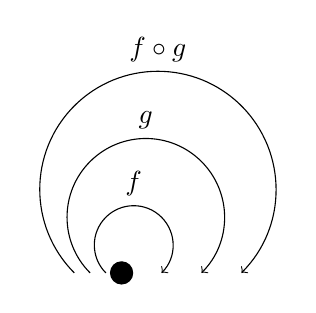
\begin{tikzpicture}
\filldraw (0, 0) circle (4pt) node (obj) {};
\draw[->] (-0.2, 0) arc[radius=5mm, start angle=225, end angle=-45] node[pos=0.5, above]{$f$};
\draw[->] (-0.4, 0) arc[radius=10mm, start angle=225, end angle=-45] node[pos=0.5, above]{$g$};
\draw[->] (-0.6, 0) arc[radius=15mm, start angle=225, end angle=-45] node[pos=0.5, above]{$f \circ g$};
\end{tikzpicture}
\caption{The monoid category with only one object}
\label{fig:monoid-as-category}
\end{figure}

\index{Monoid category}
For monoid, we see both the category $\pmb{Mon}$, that contains all the monoids in the universe, and the category with only one monoid. It is like a hidden world in a piece of sand. What's more interesting, for any object $A$ in a category $\pmb{C}$, define set $hom(A, A)$ as all the arrows from $A$ to $A$ itself. Then this set of arrows forms a monoid under composite operation, where the identity element is the identity arrow. Such symmetry emerges surprisingly.

\index{Category of sets under total functions}
Our second example is set. Let every set be an object\footnote{Whenever consider the set of all sets, it ends up of Russel's paradox `the set all sets that does not contain itself'. We'll revisit Russel's paradox in chapter 7.}, the arrow is a function (or map) from one set $A$ to another set $B$. We call $A$ the domain of definition, and $B$ is the domain of the function value\footnote{It is total function, which can be applied to every elements in domain $A$.}. The composition is function composite. For functions $y = f(x)$ and $z = g(y)$, their composition is $z = (g \circ f)(x) = g(f(x))$. It's easy to verify that function composition is associative. The identity element is the identity function $id(x) = x$. Hence we obtain the category $\pmb{Set}$ of all sets and functions.

\index{partial order set} \index{poset}
\index{pre-order set} \index{preset}
Our third example contains a pair of concepts. {\em partial order set} and {\em pre-order set}. Given a set, pre-order means we can compare every two elements in it. We often use the symbol $\leq$ to represent this binary relation. It does not necessarily mean less than or equal relation between numbers, it can mean one set is subset of the other, one string is post-fix of the other, one person is descendant of the other etc. If the relation $\leq$ satisfies the following conditions, we call it a pre-order:

\begin{itemize}
\item \textbf{reflexive}: For every element $a$ in the set, we have $a \leq a$;
\item \textbf{transitive}: If $a \leq b$ and $b \leq c$, then $a \leq c$;
\end{itemize}

On top of these two, if the relation is also anti-symmetric, we call it partial order:

\begin{itemize}
\item \textbf{anti-symmetric}: if $a \leq b$ and $b \leq a$, then $a = b$;
\end{itemize}

We define the set satisfies pre-oder, and the set satisfies partial order as:

\[
preset \quad \quad \quad poset
\]

\begin{figure}[htbp]
\centering
\begin{tikzpicture}[scale=0.5]
  \matrix (m) [matrix of math nodes,
               row sep=1em, column sep=1em, minimum width=2em]{
     % 4 row x 6 column
     & \shortstack{Old ``Scotty'' \\ McDuck} & & & \shortstack{Grandma \\ Duck} & \\
     \shortstack{Scrooge \\ McDuck} & \shortstack{Matilda \\ McDuck} & \shortstack{Goosetail \\ Gander} & \shortstack{Hortense \\ McDuck} & \shortstack{Quackmore \\ Duck} & \shortstack{Daphne \\ Duck} \\
     & & \shortstack{Gladstone \\ Gander} & \shortstack{Donald \\ Duck} & \shortstack{Thelma \\ Duck} & \\
     & & & \text{Huey} & \text{Dewey} & \text{Louie} \\};
  \path[<-]
    (m-1-2) edge (m-2-1) % Scotty -- Scrooge
    (m-1-2) edge (m-2-2) % Scotty -- Matilda
    (m-1-2) edge (m-2-4) % Scotty -- Hortense
    (m-1-5) edge (m-2-5) % Grandma -- Quackmore
    (m-1-5) edge (m-2-6) % Grandma -- Daphne
    (m-2-3) edge (m-3-3) % Goosetail -- Gladstone
    (m-2-5) edge (m-3-4) % Quackmore -- Donald
    (m-2-5) edge (m-3-5) % Quackmore -- Thelma
    (m-3-5) edge (m-4-4) % Thelma -- Huey
    (m-3-5) edge (m-4-5) % Thelma -- Dewey
    (m-3-5) edge (m-4-6); % Thelma -- Louie
\end{tikzpicture}
\caption{Duck family tree}
\label{fig:genealogical-tree}
\end{figure}

Not every two elements are comparable in partial order set. The figures in Duck Donald family form a partial order set under the descendant relation, as shown in figure \ref{fig:genealogical-tree}. We can see Donald$\leq$Quackmore, but there is no $\leq$ relation between Huey and Donald, or between Donald and Scrooge. Although every one has its ancestor in this family tree (The figures at the root can be considered as the ancestor of themselves according to reflexive rule), but the figures at the same level or in different branches are not comparable.

As shown in \ref{fig:powerset}, for a given set $\{x, y, z\}$, all its subsets form a partial order set under the inclusion relationship. Although every element (a subset) has a subset, elements at the same level are not comparable. Besides that there are also non-comparable elements, like $\{x\}$ and $\{y, z\}$ for example.

\begin{figure}[htbp]
 \centering
 \includegraphics[scale=0.4]{img/powerset.png}
 %\captionsetup{labelformat=empty}
 \caption{All subsets form a partial order set under inclusion relationship.}
 \label{fig:powerset}
\end{figure}

\index{category of partial order set} \index{category of pre-order set}
In general, any partial order set is a pre-order set, but the reverse is not necessarily true. A pre-order set may not be partial order set. We learn monotone function in high school math. Monotone function never decreases, if $x \leq y$, then $f(x) \leq f(y)$. By composing monotone functions on top of partial order set or pre-order set, we obtain a pair of categories.

\[
\pmb{Pre} \quad \quad \quad \pmb{Pos}
\]

The objects are all $presets$ and $posets$, the arrows are monotone maps. As the identity map is also monotone, it is the identity arrow in the category.

We intend to choose categories of monoids and pre-set as two examples. They are the two most simple categories. The study of monoids is the study of composition in the miniature. The study of presets is the study of comparison in the miniature. It is the core of the entire category to study the composition and comparison of mathematical structures. In a sense every category is an amalgam of certain monoids and presets(\cite{Simmons2011}, p13).

$\pmb{Pre}$ is a big category that contains all the pre-order sets in the world. On the other hand, preset category can also be very small, that only contains one pre-order set. Consider the set of elements $i, j, k, ...$, if $i$ and $j$ are comparable, and $i \leq j$, we define

\[
i \longrightarrow j
\]

Hence for every two objects, either there is no arrow between them, which means they are not comparable; or there exists one, which means there is $\leq$ relationship. In summary, there is at most one arrow between any two objects. We can verify that such arrows are composable, and for every element $i$, relation $i \leq i$ holds, hence there exists self-pointed arrow. Such preset itself forms a category. Again, we see the symmetry between preset and monoid categories. Monoid category contains only one object, but has many arrows; while preset category contains many objects, but has at most one arrow between objects.

\begin{Exercise}
\Question{Prove that the identity arrow is unique (hint: refer to the uniqueness of identity element for groups in previous chapter).}
\Question{Verify the monoid $(S, \cup, \varnothing)$ (the elements are sets, the binary operation is set union, the identity element is empty set) and $(N, +, 0)$ (elements are natural numbers, the binary operation is add, the identity element is zero) are all categories that contain only one object.}
\Question{In chapter 1, we introduced Peano's axioms for natural numbers and the isomorphic structures to Peano arithmetic, like the linked-list etc. They can be described in categories. This was found by German mathematician Richard Dedekind although the category theory was not established by his time. We named this category as Peano category, denoted as $\pmb{Pno}$. The objects in this category is $(A, f, z)$, where $A$ is a set, for example natural numbers $N$; $f: A \to A$ is a successor function. It is $succ$ for natural numbers; $z \in A$ is the starting element, it is zero for natural numbers. Given any two Peano objects $(A, f, z)$ and $(B, g, c)$, define the morphism from $A$ to $B$ as:

\[
A \arrowto{\phi} B
\]

It satisfies:

\[
\phi \circ f = g \circ \phi \quad \text{and} \quad \phi(z) = c
\]

Verify that $\pmb{Pno}$ is a category.}
\end{Exercise}

\subsection{Arrow $\neq$ function}

In most examples so far, arrows are either functions, or function like things, such as maps or morphisms. It gives us an illusion that arrows mean function like things. The next example helps us to realize such deception. There is a relation category. The objects are sets. The arrow from set $A$ to set $B$, $A \arrowto{R} B$ is defined as:

\[
R \subseteq B \times A
\]

Let's see what does it mean. Set $B \times A$ represents all element combinations from $B$ and $A$. It is called the product of $B$ and $A$:

\[
B \times A = \{(b, a) | b \in B, a \in A\}
\]

Use the Donald Duck family for example, set $A =$ \{ Scrooge McDuck, Matilda McDuck, Hortense McDuck\} contains three members in McDuck family, set $B = $ \{Goosetail Gander, Quackmore Duck\} contains two external members, then the product of $B \times A$ is \{(Goosetail Gander, Scrooge McDuck),(Goosetail Gander, Matilda McDuck), (Goosetail Gander, Hortense McDuck), (Quackmore Duck, Scrooge McDuck), (Quackmore Duck, Matilda McDuck), (Quackmore Duck, Hortense MuDuck)\}. Set $R$ is a subset of $B \times A$, it represents some relation between $A$ and $B$. If element $a$ in $A$, and element $b$ in $B$ satisfy relation $R$, then $(b, a) \in R$, we denote it as $bRa$. For this example, we can let $R=$ \{(Goosetail Gander, Matilda McDuck), (Quackmore Duck, Hortense MuDuck)\}, then $R$ means they are couples (In Donald Duck story, Goosetail married Matilda, they adopted Gladstone as their child; Quackmore married Hortense, they are parents of Donald).

Hence the set of {\em all} arrows from $A$ to $B$ represents all possible relations from $A$ to $B$. Let's consider the arrow composition:

\[
A \to B \to C
\]

If there exists an element $b$ in some intermediate set, that both relations $bRa$ and $cSb$ hold, we say there is composition between arrows. Use the Donald Duck family for example. Let set $C=$ = \{Gladstone, Donald, Thelma\}. Relation $S=$ \{(Donald, Quackmore), (Thelma, Quackmore)\} means son and father. Thus the composite arrow $S \circ R$ gives result \{(Donald, Hortense), (Thelma, Hortense)\}, it means the relation that $c$ is the son of mother $a$. Hence both relations are satisfied through Quackmore, so that Donald and Thelma are sons of their mother Hortense. The definition of identity arrow is simple, every element has an identical relation to itself.

We can generate a new category from any existing category, for example, by reversing the arrows in category $\pmb{C}$, we obtained a dual {\em opposite} category $\pmb{C}^{op}$. Hence when we understand a category, we understand its dual category as well.

\section{Functors}

We mentioned category theory is the `second' level abstraction on top of algebraic structure. We've seen how to abstract all sets and maps, groups and morphisms, posets and monotone functions into categories. The next question is how to bridge these categories and compare them? Functor\footnote{Some C++ programming language materials use functor to name function object. It has nothing related to category theory.} is used to compare categories and their inner relations (objects and arrows).

\subsection{Definition of functor}
\index{functor}
In some sense, functor can be considered as the transform (morphism) between categories. However, it does not only map the object from one category to the other, but also maps the arrow. This makes functor different from the normal morphism (between groups for example).

We often use $\mathbf{F}$ to denote functor. Since functor likes the morphism for category, it must faithfully preserve the structure and relations between categories. In order to achieve this, a functor need satisfy two conditions:

\begin{enumerate}
\item Any identity arrow in one category is transformed to identity arrow in another category. As shown in below figure:

\[
A \arrowto{id} A \quad \longmapsto \quad \mathbf{F}A \arrowto{id} \mathbf{F}A
\]

\index{covariance} \index{contravariance}
\item Any composition of arrows in one category is transformed to composition in another category\footnote{There are two different types of transformation, one is called covariance, the other is contravariance. The two terms are also used in programming language type system. We only consider covariance in this book}.

\begin{center}
\begin{tikzpicture}
  \matrix (m) [matrix of math nodes,
               row sep=2em, column sep=2.5em, minimum width=2em]{
       & B &   & \longmapsto &             & \mathbf{F}B & \\
     A &   & C & \text{covariance} & \mathbf{F}A &  & \mathbf{F}C\\};
  \path[-stealth]
    (m-2-1) edge node [above] {$f$} (m-1-2)
    (m-1-2) edge node [above] {$g$} (m-2-3)
    (m-2-1) edge node [below] {$g \circ f$} (m-2-3)
    (m-2-5) edge node [above] {$\mathbf{F}(f)$} (m-1-6)
    (m-1-6) edge node [above] {$\mathbf{F}(g)$} (m-2-7)
    (m-2-5) edge node [below] {$\mathbf{F}(g \circ f)$} (m-2-7);
\end{tikzpicture}
\end{center}

\[
\mathbf{F}(g \circ f) = \mathbf{F}(g) \circ \mathbf{F}(f)
\]
\end{enumerate}

In summary, functor preserves identity morphisms and composition of morphisms. Functors can also be composited, for example functor $(\mathbf{F} \mathbf{G})(f)$ means first apply $\mathbf{G}$ on arrow $f$, then apply $\mathbf{F}$ on top of the arrow in the new category.

\subsection{Functor examples}
\label{sec:functor:examples}

\begin{wrapfigure}{R}{0.3\textwidth}
 \centering
 \includegraphics[scale=0.3]{img/blackhole.jpg}
 \captionsetup{labelformat=empty}
 \caption{Constant functor acts like a blackhole.}
 \label{fig:blackhole}
\end{wrapfigure}

\index{functor!identity functor} \index{functor!id functor}
Let's use some examples to understand functor. If a functor maps a category to itself, it is called {\em endo-functor}\footnote{Similar to the automorphism in abstract algebra, which we introduced in previous chapter.}. The simplest functor is the identity functor, which is an endo-functor, denoted as $id: \pmb{C} \to \pmb{C}$. It can be applied to any category, maps object $A$ to $A$, and maps arrow $f$ to $f$.

\index{functor!constant functor}
The second simplest functor is the constant functor. It acts like a blackhole. We denote it as $\mathbf{K}_B : \pmb{C} \to \pmb{B}$. It can be applied to any category, maps all objects to the blackhole object $B$, and maps all arrows to the identity arrow in the blackhole $id_B$. The blackhole category has only one identity arrow, it also satisfy the arrow composition condition: $id_B \circ id_B = id_B$.

\begin{example}
\normalfont
\index{functor!maybe functor}
Maybe functor. Computer scientist, Tony Hoare (Sir Charles Antony Richard Hoare), who developed the quicksort algorithm, and awarded ACM Turing award in 1980, had an interesting speaking apologised for inventing the null reference\footnote{At a software conference called QCon London in 2009}.

%\begin{wrapfigure}{L}{0.25\textwidth}
\begin{figure}[htbp]
 \centering
 \includegraphics[scale=1]{img/Hoare.jpg}
 \captionsetup{labelformat=empty}
 \caption{Tony Hoare}
 \label{fig:Hoare}
\end{figure}
%\end{wrapfigure}

\begin{quotation}
\itshape
I call it my billion-dollar mistake. It was the invention of the null reference in 1965. At that time, I was designing the first comprehensive type system for references in an object oriented language (ALGOL W). My goal was to ensure that all use of references should be absolutely safe, with checking performed automatically by the compiler. But I couldn't resist the temptation to put in a null reference, simply because it was so easy to implement. This has led to innumerable errors, vulnerabilities, and system crashes, which have probably caused a billion dollars of pain and damage in the last forty years\cite{Wiki-Hoare}.
\end{quotation}

After 2015, the mainstream programming environments gradually adopted the maybe concept to replace the error prone null\footnote{For example the \texttt{Optional<T>} in Java and C++}.

Below diagram illustrates how $\mathbf{Maybe}$ behaves.

\begin{center}
\begin{tikzpicture}
  \matrix (m) [matrix of math nodes,
               row sep=2em, column sep=2.5em, minimum width=2em]{
     A & \mathbf{Maybe}\ A \\
     B & \mathbf{Maybe}\ B \\};
  \path[-stealth]
    (m-1-1) edge (m-1-2)
    (m-2-1) edge (m-2-2)
    (m-1-1) edge node [left] {$f$} (m-2-1)
    (m-1-2) edge node [right] {$\mathbf{Maybe}(f)$} (m-2-2);
\end{tikzpicture}
\end{center}

The left side objects $A$ and $B$ can be data types, like integer, Boolean. While the right side objects are mapped types through functor $\mathbf{Maybe}$. If $A$ represents $Int$, then the right side corresponds to $\mathbf{Maybe}\ Int$, if $B$ represents $Bool$, then the right side corresponds to $\mathbf{Maybe}\ Bool$. How does the maybe functor map objects? that part is defined as:

\lstset{frame=none}
\begin{lstlisting}
data Maybe A = Nothing | Just A
\end{lstlisting}

It means, if the object is type $A$, then the mapped object is type $\mathbf{Maybe}\ A$. Note the object is type, but not value. The value of $\mathbf{Maybe}\ A$ is either empty, denoted as $Nothing$, or a value constructed by $Just$.

Use type $Int$ for example, through the maybe functor, it is mapped to $\mathbf{Maybe}\ Int$. The value could be $Nothing$ or $Just\ 5$ for instance.

Consider a binary search tree, that contains elements of type $A$. When search a value in the tree, it may not be found, therefore the type of search result is $\mathbf{Maybe}\ A$\footnote{The complete example program can be found in the appendix of this chapter}.

\[
\begin{array}{rcl}
lookup\ Nil\ \_ & = & Nothing \\
lookup\ (Br\ l\ k\ r)\ x & = & \begin{cases}
  x < k: & lookup\ l\ x \\
  x > k: & lookup\ r\ x \\
  x = k: & Just\ k
\end{cases}
\end{array}
\]

For $\mathbf{Maybe}$ type data, we must handle two different possible values, for example:

\[
\begin{array}{lcl}
elem\ Nothing & = & False \\
elem\ (Just\ x) & = & True
\end{array}
\]

Functor maps object, and also maps arrow. We see how $\mathbf{Maybe}$ functor maps object. How does it map arrow? On the left side in above diagram, there is an up-down arrow $A \arrowto{f} B$, and there is also an arrow $\mathbf{Maybe}\ A \arrowto{\mathbf{Maybe}(f)} \mathbf{Maybe}\ B$ on the right side. Let's name the right side arrow $f'$. If we know the behavior of the left side arrow $f$, then what does the right side arrow behave? We mentioned for $\mathbf{Maybe}$ type data, we must handle two different possible values, hence $f'$ should behave like this:

\[
\begin{array}{lcl}
f'\ Nothing & = & Nothing \\
f'\ (Just\ x) & = & Just\ (f\ x)
\end{array}
\]

\index{fmap}
For given $f$, maps to $f'$, it is exactly what $\mathbf{Maybe}$ functor does for an arrow. In programming environment, we often use $fmap$ to define the map for arrow. We can define every functor $\mathbf{F}$ satisfies:

\[
fmap : (A \to B) \to (\mathbf{F} A \to \mathbf{F} B)
\]

For functor $\mathbf{F}$, it maps the arrow from $A$ to $B$ to the arrow from $\mathbf{F} A$ to $\mathbf{F} B$. Hence for $\mathbf{Maybe}$ functor, the corresponding $fmap$ is defined as below:

\[
\begin{array}{l}
\quad    fmap : (A \to B) \to (\mathbf{Maybe}\ A \to \mathbf{Maybe}\ B) \\
\quad    fmap\ f\ Nothing = Nothing \\
\quad    fmap\ f\ (Just\ x) = Just\ (f\ x) \\
\end{array}
\]

Back to the binary search tree example, if the elements in the tree are integers, we want to search a value, and convert it to binary format if find; otherwise return $Nothing$. Suppose there has already existed a function that converts a decimal number to its binary format:

\[
binary(n) = \begin{cases}
n < 2: & [n] \\
\text{Otherwise}: & binary(\lfloor\dfrac{n}{2}\rfloor)\doubleplus[n \bmod 2]
\end{cases}
\]

Here is the corresponding example program. It uses tail recursion for performance purpose.

\lstset{frame=single}
\begin{lstlisting}[style=Haskell]
binary = bin [] where
   bin xs 0 = 0 : xs
   bin xs 1 = 1 : xs
   bin xs n = bin ((n `mod` 2) : xs) (n `div` 2)
\end{lstlisting}

With functor, we can `lift' this function arrow up as shown in below diagram:

\begin{center}
\begin{tikzpicture}
  \matrix (m) [matrix of math nodes,
               row sep=2em, column sep=6em, minimum width=2em]{
     \mathbf{Maybe}\ Int & \mathbf{Maybe}\ [Int] \\
     Int & \left [ Int \right] \\};
  \path[-stealth]
    (m-1-1) edge node [above] {$fmap\ binary$} (m-1-2)
    (m-2-1) edge node [below] {$binary$} (m-2-2)
    (m-2-1) edge (m-1-1)
    (m-2-2) edge (m-1-2);
\end{tikzpicture}
\end{center}

Hence, we directly use maybe functor and $binary$ arrow to manipulate the search result from the tree:

\[
fmap\ binary\ (lookup\ t\ x)
\]

We can consider there are two worlds in above diagram. The bottom is the world on the earth, threatened by the null reference; the upper is the world in the sky, free from null and safe. With maybe functor, all the legacy programs on the earth, even they are not capable to handle null, can be lift to the sky, to the safe world dominated by the maybe functor.

\begin{mdframed}
\begin{proof}
\textbf{Readers can skip the contents in this box} To verify Maybe is a functor, we need check the two conditions about arrow mapping:

\[
\begin{array}{l}
fmap\ id = id \\
fmap\ (f \circ g) = fmap\ f \circ fmap\ g
\end{array}
\]

For the first condition, the definition of $id$ is:

\[
id\ x = x
\]

Therefore:

\[
\begin{array}{rcll}
fmap\ id\ Nothing & = & Nothing & \text{definition of $fmap$} \\
                  & = & id\ Nothing & \text{reverse of $id$} \\
\end{array}
\]

And

\[
\begin{array}{rcll}
fmap\ id\ (Just\ x) & = & Just\ (id\ x) & \text{definition of $fmap$} \\
                    & = & Just\ x & \text{definition of $id$} \\
                    & = & id\ (Just\ x) & \text{reverse of $id$}
\end{array}
\]

For the second condition:

\[
\resizebox{\textwidth}{!}{\ensuremath{
\begin{array}{rcll}
fmap\ (f \circ g)\ Nothing & = & Nothing & \text{definition of $fmap$} \\
           & = & fmap\ f\ Nothing & \text{reverse of $fmap$} \\
           & = & fmap\ f\ (fmap\ g\ Nothing) & \text{reverse of $fmap$} \\
           & = & (fmap\ f\ \circ fmap\ g)\ Nothing & \text{reverse of function composition}
\end{array}
}}
\]

And

\[
\resizebox{\textwidth}{!}{\ensuremath{
\begin{array}{rcll}
fmap\ (f \circ g)\ (Just\ x) & = & Just\ ((f \circ g)\ x) & \text{definition of $fmap$} \\
           & = & Just\ (f\ (g\ x)) & \text{function composition} \\
           & = & fmap\ f\ (Just\ (g\ x)) & \text{reverse of $fmap$} \\
           & = & fmap\ f\ (fmap\ g\ (Just\ x)) & \text{reverse of $fmap$} \\
           & = & (fmap\ f\ \circ fmap\ g)\ (Just\ x) & \text{reverse of function composition}
\end{array}
}}
\]

Therefore, Maybe is really a functor.
\end{proof}
\end{mdframed}
\end{example}

\begin{example}
\normalfont
\index{functor!list functor}
List functor. We introduced the definition of list in chapter 1 as:

\lstset{frame=none}
\begin{lstlisting}
data List A = Nil | Cons(A, List A)
\end{lstlisting}

From programming perspective, it defines the linked-list data structure. The elements stored are of type $A$. We call it link-list of type $A$. From category perspective, a list functor need define maps for both object and arrow. Here objects are types, arrows are total functions. Below diagram illustrates how list functor behaves.

\begin{center}
\begin{tikzpicture}
  \matrix (m) [matrix of math nodes,
               row sep=2em, column sep=2.5em, minimum width=2em]{
     A & \mathbf{List}\ A \\
     B & \mathbf{List}\ B \\};
  \path[-stealth]
    (m-1-1) edge (m-1-2)
    (m-2-1) edge (m-2-2)
    (m-1-1) edge node [left] {$f$} (m-2-1)
    (m-1-2) edge node [right] {$\mathbf{List}(f)$} (m-2-2);
\end{tikzpicture}
\end{center}

Objects $A, B$ on the left side are data types, like integer, Boolean, or even complex types such as $\mathbf{Maybe}\ Char$. Objects on the right side, are types mapped by list functor. If $A$ is integer type $Int$, then the right side corresponds to $\mathbf{List}\ Int$; if $B$ is character type $Char$, then the right side corresponds to $\mathbf{List}\ Char$, which is $String$ essentially.

We highlight again that here the object is type, but not value. $A$ can be $Int$, but can not be 5, a particular value. Hence $\mathbf{List}\ A$ corresponds to list of integers, but not a particular list, like [1, 1, 2, 3, 5]. How to generate list values? Function $Nil$ and $Cons$ are used to generate empty list or list like $List(1, List(1, List(2, Nil)))$.

Now we know how list functor maps objects. But how does it map arrows? Given a function $f: A \to B$, how to obtain another function $g: \mathbf{List}\ A \to \mathbf{List}\ B$ through list functor? Similar to maybe functor, we can realize $fmap$ to map arrow $f$ to arrow $g$. The type signature for list functor is:

\[
fmap: (A \to B) \to (\mathbf{List}\ A \to \mathbf{List}\ B)
\]

Let's consider how $g$ behaves. For the simplest case, no matter how $f$ is defined, if the value of $\mathbf{List}\ A$ is an empty list $Nil$, then applying $g$ on it gives empty list anyway. Therefore:

\[
fmap\ f\ Nil = Nil
\]

For the recursive case $Cons(x, xs)$, where $x$ is some value of type $A$, and $xs$ is a sub-list of type $\mathbf{List}\ A$. If $f(x) = y$, which maps $x$ of type $A$ to $y$ of type $B$, then we first apply $f$ to $x$, next recursively apply it to the sub-list $xs$ to obtain a new sub-list $ys$ with the element type of $B$. Finally, we concatenate $y$ and $ys$ as the result:

\[
fmap\ f\ Cons(x, xs) = Cons(f\ x, fmap\ f\ xs)
\]

Summarize them together, we have the complete definition of $fmap$ for list:

\[
\begin{array}{l}
\quad    fmap : (A \to B) \to (\mathbf{List}\ A \to \mathbf{List}\ B) \\
\quad    fmap\ f\ Nil = Nil \\
\quad    fmap\ f\ Cons(x, xs) = Cons(f\ x, fmap\ f\ xs) \\
\end{array}
\]

In chapter 1, we introduced the simplified notation, using the infix `:' for $Cons$, and `[]' for $Nil$, then the definition of list functor that maps arrows can be simplified as:

\[
\begin{array}{l}
\quad    fmap : (A \to B) \to (\mathbf{List}\ A \to \mathbf{List}\ B) \\
\quad    fmap\ f\ [] = [] \\
\quad    fmap\ f\ (x:xs) = (f\ x):(fmap\ f\ xs) \\
\end{array}
\]

Compare this definition with the list mapping definition in chapter 1, we find they are exactly same except for the name. It means we can re-use the list mapping to define list functor. This is the case in some programming environment, which re-uses \texttt{map} for list functor.

\lstset{frame=single}
\begin{lstlisting}
instance Functor [] where
    fmap = map
\end{lstlisting}

\begin{mdframed}
At the end of this example, let's verify the arrow mapping for list functor preserve identity and composition. \textbf{Readers can skip the proof in this box}.

\[
\begin{array}{l}
fmap\ id = id \\
fmap\ (f \circ g) = fmap\ f \circ fmap\ g
\end{array}
\]

\begin{proof}
We use mathematical induction to verify the identity condition. First for empty list:

\[
\begin{array}{rcll}
fmap\ id\ Nil & = & Nil & \text{definition of $fmap$} \\
              & = & id\ Nil & \text{reverse of $id$} \\
\end{array}
\]

For the recursive case of $(x:xs)$, assume $fmap\ id\ xs = id\ xs$ holds, we have:

\[
\begin{array}{rcll}
fmap\ id\ (x:xs) & = & (id\ x):(fmap\ id\ xs) & \text{definition of $fmap$} \\
                 & = & (id\ x):(id\ xs) & \text{induction assumption} \\
                 & = & x:xs & \text{definition of $id$} \\
                 & = & id\ (x:xs) & \text{reverse of $id$}
\end{array}
\]

Again, we use mathematical induction to verify composition condition. For empty list, we have:

\[
\begin{array}{rcll}
fmap\ (f \circ g)\ Nil & = & Nil & \text{definition of $fmap$} \\
           & = & fmap\ f\ Nil & \text{reverse of $fmap$} \\
           & = & fmap\ f\ (fmap\ g\ Nil) & \text{reverse of $fmap$} \\
           & = & (fmap\ f\ \circ fmap\ g)\ Nil & \text{reverse of function composition}
\end{array}
\]

For the recursive case of $(x:xs)$, assume $fmap\ (f \circ g)\ xs = (fmap\ f \circ fmap\ g)\ xs$ holds, we have:

\[
\resizebox{\textwidth}{!}{\ensuremath{
\begin{array}{rcll}
fmap\ (f \circ g)\ (x:xs) & = & ((f \circ g)\ x):(fmap\ (f \circ g)\ xs) & \text{definition of $fmap$} \\
  & = & ((f \circ g)\ x):((fmap\ f \circ fmap\ g)\ xs) & \text{induction assumption} \\
  & = & (f(g\ x)):(fmap\ f\ (fmap\ g\ xs)) & \text{function composition} \\
  & = & fmap\ f\ ((g\ x):(fmap\ g\ xs)) & \text{reverse of $fmap$} \\
  & = & fmap\ f\ (fmap\ g\ (x:xs)) & \text{reverse of $fmap$ again} \\
  & = & (fmap\ f\ \circ fmap\ g)\ (x:xs) & \text{reverse of function composition}
\end{array}
}}
\]

Thus we verified $\mathbf{List}$ is really a functor.
\end{proof}
\end{mdframed}
\end{example}

\begin{Exercise}
\Question{For the list functor, define the arrow map with $foldr$.}
\Question{Verify that the composition of maybe functor and list functor $\mathbf{Maybe} \circ \mathbf{List}$ and $\mathbf{List} \circ \mathbf{Maybe}$ are all functors.}
\Question{Proof that the composition for any functors $\mathbf{G} \circ \mathbf{F}$ is still a functor.}
\Question{Give an example functor for preset.}
\Question{For the binary tree defined in chapter 2, define the functor for it.}
\end{Exercise}

\section{Products and coproducts}

Before we introduce more complex categories and functors, let us see what product and coproduct are. We start from the product of sets. Given two set $A$ and $B$, their Cartesian product $A \times B$ is the set of all ordered pairs $(a, b)$, where $a \in A$ and $b \in B$:

\[
\{(a, b) | a \in A, b \in B\}
\]

For example, the product of finite sets $\{1, 2, 3\}$ and $\{a, b\}$ is:

\[
\{(1, a), (2, a), (3, a), (1, b), (2, b), (3, b)\}
\]

If set $A$ and $B$ are the same algebraic structures, like group, ring etc., then we can define objects and arrows as shown in below diagram:

\begin{center}
\begin{tikzpicture}
  \matrix (m) [matrix of math nodes,
               row sep=2em, column sep=2em, minimum width=2em]{
      &   & (a, b) &  & \\
      &   & A \times B & & \\
      &   &            & & \\
    a & A &            & B & b \\};
  \path[|->]
    (m-1-3) edge (m-4-1)
    (m-1-3) edge (m-4-5);
  \path[-stealth]
    (m-2-3) edge (m-4-2)
    (m-2-3) edge (m-4-4);
\end{tikzpicture}
\end{center}

%\begin{wrapfigure}{L}{0.25\textwidth}
\begin{figure}[htbp]
 \centering
 \includegraphics[scale=0.2]{img/Descartes.jpg}
 \captionsetup{labelformat=empty}
 \caption{René Descartes (1596 - 1650). Portrait after Frans Hals, oil on canvas, Louvre Museum}
 \label{fig:Decartes}
\end{figure}
%\end{wrapfigure}

\index{Cartesian product} \index{Descartes}
Cartesian product, also known as direct product, is named after René Descartes, the great French philosopher, mathematician, and scientist. In the days of Descartes, Latin was a widely used academy language. He also had a Latinized name: Renatus Cartesius. Its adjective form is Cartesian. This is the reason why we say Cartesian product or Cartesian coordinate system today.

Descartes was born in La Haye, near Tours, France in 1596. His father was a member of the Parlement of Brittany at Rennes. His mother died a year after giving birth to him, and so he was not expected to survive. His father then remarried in 1600. Descartes lived with his grandmother at La Haye. His health was poor when he was a child. Throughout his childhood, up to his twenties, he was pale and had a persistent cough which was probably due to tuberculosis. It seems likely that he inherited these health problems from his mother.

In 1607, he entered the Jesuit college of La Flèche, where he was introduced to mathematics and physics, including Galileo's work. While in the school his health was poor and, instead of rising at 5 AM. like the other boys, he was granted permission to remain in bed until 11 o'clock in the morning, a custom he maintained until the year of his death.

After graduation in 1614, he studied for two years at the University of Poitiers. He received a law degree in 1616 to comply with his father's wishes but he quickly decided that this was not the path he wanted to follow. He returned to Paris, then became a volunteer in the army of Maurice of Nassau. In the army, Descartes started studying mathematics and mechanics under the Dutch scientist Isaac Beeckman, and began to seek a unified science of nature.

After this time in Holland he left the service of Maurice of Nassau and travelled through Europe. In 1619 he joined the Bavarian army and was stationed in Ulm. An important event in his life was three dreams he had in November 1619. These he believed were sent by a divine spirit with the intention of revealing to him a new approach to philosophy. The ideas from these dreams would dominate much of his work from that time on.

From 1620 to 1628 Descartes travelled through Europe, spending time in Bohemia, Hungary, Germany, Holland, through Switzerland to Italy, then Venice and Rome. He returned Paris in 1625. His Paris home became a meeting place for philosophers and mathematicians and steadily became more and more busy. By 1628 Descartes, tired of the bustle of Paris, the house full of people, and of the life of travelling he had before, decided to settle down where he could work in solitude. He gave much thought to choosing a country suited to his nature and he chose Holland. What he longed for was somewhere peaceful where he could work away from the distractions of a city such as Paris yet still have access to the facilities of a city. It was a good decision which he did not seem to regret over the next twenty years. He told his friend Marin Mersenne\footnote{Mersenne was a French polymath, whose works touched a wide variety of fields. He is perhaps best known today among mathematicians for Mersenne prime numbers, in the form $M_n = 2^n − 1$ for some integer $n$. He had many contacts in the scientific world and has been called "the center of the world of science and mathematics during the first half of the 1600s".} where he was living so that he might keep in touch with the mathematical world, but otherwise he kept his place of residence a secret. Descartes wrote all his major work during his 20-plus years in the Netherlands, initiating a revolution in mathematics and philosophy. In 1633, Galileo was condemned by the Italian Inquisition, and Descartes abandoned plans to publish {\em Treatise on the World}, his work of the previous four years. Nevertheless, in 1637 he published parts of this work in three essays: {\em The Meteors}, {\em Dioptrics} and {\em Geometry}, preceded by an introduction, his famous {\em Discourse on the Method}.

In {\em Geometry}, Descartes exploited the discoveries he made with Pierre de Fermat. This later became known as Cartesian Geometry. Descartes continued to publish works concerning both mathematics and philosophy for the rest of his life. In 1641 he published a metaphysics treatise, {\em Meditations on First Philosophy}. It was followed in 1644 by {\em Principles of Philosophy}. He became the most influential philosophers in Europe.

In 1649 Queen Christina of Sweden persuaded Descartes to go to Stockholm. However the Queen wanted to draw tangents at 5 AM. and Descartes broke the habit of his lifetime of getting up at 11 o'clock. After only a few months in the cold northern climate, walking to the palace for 5 o'clock every morning, he died of pneumonia February 1650 at the age of 54.

Descartes left the best known philosophical statement ``I think, therefore I am'' (French: Je pense, donc je suis; Latin: cogito, ergo sum). Descartes laid the foundation for 17th-century continental rationalism. He was well-versed in mathematics as well as philosophy, and contributed greatly to science as well. He is credited as the father of analytical geometry, the bridge between algebra and geometry—used in the discovery of infinitesimal calculus and analysis. Descartes was also one of the key figures in the Scientific Revolution.

\vspace{5mm}

Symmetric to the Cartesian product of sets, there is a dual construct. From two sets $A$ and $B$, we can generate a disjoint union set (sum) $A + B$. For the element in the sum, in order to know which set $A$ or $B$ it comes from, we can add a tag:

\[
A + B = (A \times \{0\}) \cup (B \times \{1\})
\]

For every element $(x, tag)$ in $A + B$, if the $tag$ is 0, we know that $x$ comes from $A$, else if the $tag$ is 1, then $x$ comes from $B$. Hence the sum of finite set $\{1, 2, 3\}$ and $\{a, b\}$ is

\[
\{(1, 0), (2, 0), (3, 0), (a, 1), (b, 1)\}
\]

When programming, $A + B$ can be defined as:

\begin{mdframed}
\[
A + B = zip\ A\ \{0, ...\} \doubleplus zip\ B\ \{1, ...\}
\]
\end{mdframed}

If set $A$ and $B$ are the same algebraic structures, we can define the below objects and arrows:

\begin{center}
\begin{tikzpicture}
  \matrix (m) [matrix of math nodes,
               row sep=2em, column sep=2em, minimum width=2em]{
    a & A &        &       &        & B & b \\
      &   &        &       &        &   & \\
      &   & (a, 0) & A + B & (b, 1) &   & \\};
  \path[|->]
    (m-1-1) edge (m-3-3)
    (m-1-7) edge (m-3-5);
  \path[-stealth]
    (m-1-2) edge (m-3-4)
    (m-1-6) edge (m-3-4);
\end{tikzpicture}
\end{center}

%\begin{wrapfigure}{R}{0.4\textwidth}
\begin{figure}[htbp]
 \centering
 \includegraphics[scale=0.06]{img/hands.png}
 \captionsetup{labelformat=empty}
 \caption{}
 \label{fig:hands}
\end{figure}
%\end{wrapfigure}

The two constructions are symmetric. If rotate the two diagrams by 90 degree, laying $A$ on top of $B$, then the two problems appear left and right. They are symmetric like our two hands. We can find a lot of such symmetric concepts in category theory. Our world is full of symmetric things. When we understand one, we understand the dual one at the same time.

\subsection{Definition of product and coproduct}
\index{product} \index{coproduct}
\begin{definition}
\normalfont
For a pair of objects $A$ and $B$ in category $\pmb{C}$, a {\em wedge}

\[
\text{to} \quad \quad \quad \text{from}
\]

\index{wedge}
the pair $A, B$ is an object $X$ together with a pair of arrows

\begin{center}
\begin{tikzpicture}
  \matrix (m) [matrix of math nodes,
               row sep=2em, column sep=2em, minimum width=2em]{
      & A &  & A & \\
    X &   &  &   & X \\
      & B &  & B & \\};
  \path[-stealth]
    (m-2-1) edge (m-1-2)
    (m-2-1) edge (m-3-2)
    (m-1-4) edge (m-2-5)
    (m-3-4) edge (m-2-5);
\end{tikzpicture}
\end{center}

in the parent category $\pmb{C}$.
\end{definition}

For a given pair of objects $A, B$ in the category, there may be many wedges on one side or the other. We look for the `best possible' wedge, the one that is as `near' the pair as possible. Technically, we look for a universal wedge. It leads to the below (pair of) definitions:

\begin{definition}
\normalfont
Given a pair object $A, B$ of a category $\pmb{C}$, a

\[
\text{product} \quad \quad \quad \text{coproduct}
\]

of the pair is a wedge:

\begin{center}
\begin{tikzpicture}
  \matrix (m) [matrix of math nodes,
               row sep=2em, column sep=2em, minimum width=2em]{
      & A &  & A & \\
    S &   &  &   & S \\
      & B &  & B & \\};
  \path[-stealth]
    (m-2-1) edge node [above] {$p_A$} (m-1-2)
    (m-2-1) edge node [below] {$p_B$} (m-3-2)
    (m-1-4) edge node [above] {$i_A$} (m-2-5)
    (m-3-4) edge node [below] {$i_B$} (m-2-5);
\end{tikzpicture}
\end{center}

with the following universal property. For each wedge

\begin{center}
\begin{tikzpicture}
  \matrix (m) [matrix of math nodes,
               row sep=2em, column sep=2em, minimum width=2em]{
      & A &  & A & \\
    X &   &  &   & X \\
      & B &  & B & \\};
  \path[-stealth]
    (m-2-1) edge node [above] {$f_A$} (m-1-2)
    (m-2-1) edge node [below] {$f_B$} (m-3-2)
    (m-1-4) edge node [above] {$f_A$} (m-2-5)
    (m-3-4) edge node [below] {$f_B$} (m-2-5);
\end{tikzpicture}
\end{center}

there is a unique arrow:

\[
 X \arrowto{m} S \quad \quad \quad S \arrowto{m} X
\]

such that,

\begin{center}
\begin{tikzpicture}
  \matrix (m) [matrix of math nodes,
               row sep=2em, column sep=2em, minimum width=2em]{
      & A &  & A & \\
    X & S &  & S & X \\
      & B &  & B & \\};
  \path[-stealth]
    % left
    (m-2-1) edge node [above] {$f_A$} (m-1-2)
    (m-2-1) edge node [below] {$f_B$} (m-3-2)
    (m-2-1) edge node [above] {$m$}   (m-2-2)
    (m-2-2) edge node [right] {$p_A$} (m-1-2)
    (m-2-2) edge node [right] {$p_B$} (m-3-2)
    % right
    (m-1-4) edge node [above] {$f_A$} (m-2-5)
    (m-3-4) edge node [below] {$f_B$} (m-2-5)
    (m-2-4) edge node [above] {$m$}   (m-2-5)
    (m-1-4) edge node [right] {$i_A$} (m-2-4)
    (m-3-4) edge node [right] {$i_B$} (m-2-4);
\end{tikzpicture}
\end{center}

\index{mediating arrow} \index{mediator}
commutes. This arrow $m$ is the {\em mediating arrow} (or mediator) for the wedge on $X$.
\end{definition}

In this definition, the product or coproduct is not just an object $S$, but an object together with a pair of arrows. For any given $X$, the mediating arrow $m$ is unique. We say the diagram commutes, it means the arrows satisfy the following equations:

\[
\begin{array}{l}
f_A = p_A \circ m \\
f_B = p_B \circ m
\end{array}
\]

It immediately leads to this special case: If $X$ equals to $S$, then $m$ is an endo-arrow (points to itself).

\[
S \arrowto{m} S
\]

Hence $m$ must be identity arrow. The diagram then simplifies to:

\begin{center}
\begin{tikzpicture}
  \matrix (m) [matrix of math nodes,
               row sep=3em, column sep=3em, minimum width=2em]{
      & A &  & A & \\
    S & S &  & S & S \\
      & B &  & B & \\};
  \path[-stealth]
    % left
    (m-2-1) edge node [above] {$p_A$} (m-1-2)
    (m-2-1) edge node [below] {$p_B$} (m-3-2)
    (m-2-1) edge node [above] {$id_S$} (m-2-2)
    (m-2-2) edge node [right] {$p_A$} (m-1-2)
    (m-2-2) edge node [right] {$p_B$} (m-3-2)
    % right
    (m-1-4) edge node [above] {$i_A$} (m-2-5)
    (m-3-4) edge node [below] {$i_B$} (m-2-5)
    (m-2-4) edge node [above] {$id_S$} (m-2-5)
    (m-1-4) edge node [right] {$i_A$} (m-2-4)
    (m-3-4) edge node [right] {$i_B$} (m-2-4);
\end{tikzpicture}
\end{center}

Among the many wedges, the product and coproduct are special, they are universal solutions. In other words, they are the `closest' or the `best' wedge. We can prove that product and coproduct are unique (see the appendix of this book). However, product and coproduct may not exist at the same time, it's also possible that neither does exist. Let's see what product and coproduct mean to set.

\begin{lemma}
\normalfont
Let $A$, $B$ be a pair of sets. Then the

\begin{center}
\begin{tabular}{ccc}
Cartesian product & \quad \quad \quad & disjoint union \\
$A \times B$ & \quad \quad \quad & $A + B$ \\
\end{tabular}
\end{center}

furnished with canonical functions form the

\begin{center}
product \quad \quad \quad coproduct
\end{center}

of the pair in the category $\pmb{Set}$.
\end{lemma}

The detailed proof can be found in the appendix of this book. In program environment, product is often realized with paired tuple $(a, b)$ and functions $fst, snd$. However, coproduct is sometimes realized with a dedicated data type.

\lstset{frame = single}
\begin{lstlisting}
data Either a b = Left a | Right b
\end{lstlisting}

The advantage is that we needn't the 0, 1 tags to mark if an element $x$ of type \texttt{Either a b} comes from \texttt{a} or \texttt{b}. The below example program handles the coproduct value through pattern matching:

\begin{lstlisting}
either :: (a -> c) -> (b -> c) -> Either a b -> c
either f _ (Left x)     =  f x
either _ g (Right y)    =  g y
\end{lstlisting}
\lstset{frame = none}

Let's see an example, consider the coproduct \texttt{Either String Int}. It is either a string, like \texttt{s = Left "hello"}; or an integer, like \texttt{n = Right 8}. If it is a string, we want to count its length; if it is a number, we want to double it. To do this, we can utilize the $either$ function: \texttt{either length (*2) x}.

Thus \texttt{either length (*2) s} will count the length of string ``hello'' which gives 5; while \texttt{either length (*2) n} will double 8 to give 16. Some programming environments have the concept of \texttt{union} or \texttt{enum} data type to realize coproduct partially. In the future, we sometimes call the two arrows of the coproduct $left$ and $right$ respectively.

\subsection{The properties of product and coproduct}

According to the definition of product and coproduct, for any wedge consist of $X$ and arrows, the mediator arrow $m$ is uniquely determined. In category $\pmb{Set}$, the mediator arrow can be defined as the following:

\[
\begin{array}{ccc}
\text{product} & & \text{coproduct} \\
m(x) = (a, b) & \quad \quad &
\begin{cases}
m (a, 0) = p(a) \\
m (b, 1) = q(b)
\end{cases}
\end{array}
\]

For a generic category, how to define the mediator arrow? To do that, we introduce two dedicated symbols for arrow operation. Given any wedge:

\begin{center}
\begin{tikzpicture}
  \matrix (m) [matrix of math nodes,
               row sep=2em, column sep=2em, minimum width=2em]{
      & A &  & A & \\
    X &   &  &   & X \\
      & B &  & B & \\};
  \path[-stealth]
    (m-2-1) edge node [above] {$f$} (m-1-2)
    (m-2-1) edge node [below] {$g$} (m-3-2)
    (m-1-4) edge node [above] {$f$} (m-2-5)
    (m-3-4) edge node [below] {$g$} (m-2-5);
\end{tikzpicture}
\end{center}

Define

\[
m = \langle f, g \rangle \quad \quad \quad m =[f, g]
\]

which satisfy:

\[
\begin{array}{rcl}
\begin{cases}
fst \circ m = f \\
snd \circ m = g
\end{cases}
& \quad \quad &
\begin{cases}
m \circ left = f \\
m \circ right = g
\end{cases}
\end{array}
\]

Hence the following diagram commutes:

\begin{center}
\begin{tikzpicture}
  \matrix (m) [matrix of math nodes,
               row sep=3em, column sep=3em, minimum width=2em]{
      & A &  & A & \\
    X & A \times B &  & A + B & X \\
      & B &  & B & \\};
  \path[-stealth]
    % left
    (m-2-1) edge node [above] {$f$} (m-1-2)
    (m-2-1) edge node [below] {$g$} (m-3-2)
    (m-2-1) edge node [above] {$\langle f, g \rangle$}   (m-2-2)
    (m-2-2) edge node [right] {$fst$} (m-1-2)
    (m-2-2) edge node [right] {$snd$} (m-3-2)
    % right
    (m-1-4) edge node [above] {$f$} (m-2-5)
    (m-3-4) edge node [below] {$g$} (m-2-5)
    (m-2-4) edge node [above] {$[f, g]$}   (m-2-5)
    (m-1-4) edge node [left] {$left$} (m-2-4)
    (m-3-4) edge node [left] {$right$} (m-2-4);
\end{tikzpicture}
\end{center}

\index{Cancellation law}
From this pair of diagrams, we can obtain some important properties for product and coproduct directly. First is the {\em cancellation law}:

\[
\begin{array}{rcl}
\begin{cases}
fst \circ \langle f, g \rangle = f \\
snd \circ \langle f, g \rangle = g
\end{cases}
& \quad \quad &
\begin{cases}
[f, g] \circ left = f \\
[f, g] \circ right = g
\end{cases}
\end{array}
\]

\index{reflection law}
For product, if arrow $f$ equals to $fst$, and arrow $g$ equals to $snd$, then we obtain the special case of identity arrow mentioned in previous section. Similarly for the coproduct, if arrow $f$ equals to $left$, and arrow $g$ equals to $right$, then the mediator arrow is also the identity arrow. We call this property the {\em reflection law}:

\[
id = \langle fst, snd \rangle \quad \quad \quad id = [left, right]
\]

If there exists another wedge $Y$ and arrows $h$ and $k$, together with $f, g$ they satisfy the following conditions:

\[
\begin{array}{ccc}
  \text{product} & & \text{coproduct} \\
  \begin{cases}
  h \circ \phi = f \\
  k \circ \phi = g
  \end{cases}
  & \quad \quad &
  \begin{cases}
  \phi \circ h = f \\
  \phi \circ k = g
  \end{cases}
\end{array}
\]

For

\[
\langle h, k \rangle \circ \phi \quad \quad \quad \phi \circ [h, k]
\]

\index{fusion law}
Substitute $m$, and apply cancellation law, then we obtain the {\em fusion law}:

\[
\begin{array}{ccc}
  \text{product} & & \text{coproduct} \\
  \begin{cases}
  h \circ \phi = f \\
  k \circ \phi = g
  \end{cases} \Rightarrow
    \langle h, k \rangle \circ \phi = \langle f, g \rangle
  & \quad \quad &
  \begin{cases}
  \phi \circ h = f \\
  \phi \circ k = g
  \end{cases} \Rightarrow
    \phi \circ [h, k] = [f, g]
\end{array}
\]

It means:

\[
\langle h, k \rangle \circ \phi = \langle h \circ \phi, k \circ \phi \rangle
\quad \quad \quad
\phi \circ [h, k] = [\phi \circ h, \phi \circ k]
\]

We'll see later, these laws play important roles during algorithm reasoning, simplification, and optimization.

\subsection{Functors from products and coproducts}
\index{bifunctor} \index{binary functor}
With product in category theory, we can introduce the concept of {\em bifunctor} (also known as binary functor). The functors we've seen so far transform the objects from one category to the objects in another category; and also transforms arrows from one category to the other. The bifunctor applies to the product of two categories $\pmb{C}$ and $\pmb{D}$. In other words, the source is $\pmb{C} \times \pmb{D}$. Bifunctor transforms objects as the following:

\[
\begin{array}{rcl}
\pmb{C} \times \pmb{D} & \longrightarrow & \pmb{E} \\
A \times B & \longmapsto & \mathbf{F}(A \times B) \\
\end{array}
\]

Besides objects, functor must transform arrows as well. For the arrow $f$ in category $\pmb{C}$, and the arrow $g$ in category $\pmb{D}$, what the bifunctor behaves? Observe the below diagram:

\begin{center}
\begin{tikzpicture}
  \matrix (m) [matrix of math nodes,
               row sep=2.5em, column sep=2.5em, minimum width=2em]{
     A & & \mathbf{F}(A \times B) \\
     C & \mathbf{F}(C \times D) & \\
       & D & B \\};
  \path[-stealth]
    (m-1-1) edge (m-1-3)
    (m-2-1) edge (m-2-2)
    (m-1-1) edge node [left] {$f$} (m-2-1)
    (m-1-3) edge node [above] {$\mathbf{F}(f \times g)$} (m-2-2)
    (m-3-2) edge (m-2-2)
    (m-3-3) edge (m-1-3)
    (m-3-3) edge node [below] {$g$} (m-3-2);
  \draw
    (-2.5, 0.5) circle[x radius=2em, y radius=4em] % C
    (0.5, -1.5) circle[x radius=5em, y radius=2em] % D
    (0.5, 0.5) circle[x radius=5.5em, y radius=3.5em]; % E
  \path
    (-2.5, -1.5) node {$\pmb{C}$}
    (1.5, -2.5) node {$\pmb{D}$}
    (3, 0.5) node {$\pmb{E}$};
\end{tikzpicture}
\end{center}

From this diagram, the arrow $A \arrowto{f} C$ and $B \arrowto{g} D$ are sent to the new arrows in category $\pmb{E}$ through the functor $\mathbf{F}$. The source object is $\mathbf{F}(A \times B)$, and the target object is $\mathbf{F}(C \times D)$. To do that, we first define the product of two arrows $f$ and $g$, it applies to the product of $A$ and $B$. For every $(a, b) \in A \times B$, it behaves as below:

\[
(f \times g)(a, b) = (f\ a\ , g\ b)
\]

The bifunctor $F$ applies to this product of arrows $f \times g$, sends it to the new arrow 头$\mathbf{F}(f \times g)$. Hence the final definition for bifunctor is as below:

\[
\begin{array}{rcl}
\pmb{C} \times \pmb{D} & \longrightarrow & \pmb{E} \\
A \times B & \longmapsto & \mathbf{F}(A \times B) \\
f \times g & \longmapsto & \mathbf{F}(f \times g) \\
\end{array}
\]

\begin{mdframed}
We need verify the bifunctor satisfies the two conditions as a functor: the identity condition and the composition condition. \textbf{Readers can skip the proof in this box}.

\[
\begin{array}{l}
\mathbf{F}(id \times id) = id \\
\mathbf{F}((f \circ f') \times (g \circ g')) = \mathbf{F}(f \times g) \circ \mathbf{F} (f' \times g')
\end{array}
\]

\begin{proof}
We treat the product as an object. If we prove the following two conditions essentially, then the proof for the bifunctor can be deduced from it through the known result of normal functors.

\[
\begin{array}{l}
id \times id = id \\
(f \circ f') \times (g \circ g') = (f \times g) \circ (f' \times g')
\end{array}
\]

We start from proving the identity condition. For all $(a, b) \in A \times B$, we have:

\[
\begin{array}{rcll}
(id \times id)(a, b) & = & (id(a), id(b)) & \text{product of arrows} \\
                     & = & (a, b) & \text{definition of $id$} \\
                     & = & id(a, b) & \text{reverse of $id$} \\
\end{array}
\]

Next we prove the composition condition.

\[
\begin{array}{rcll}
((f \circ f') \times (g \circ g'))(a, b) & = & ((f \circ f')\ a, (g \circ g')\ b) & \text{product of arrows} \\
    & = & (f(f'(a)), g(g'(b))) & \text{arrow composition} \\
    & = & (f \times g)(f'(a), g'(b)) & \text{reverse of arrows product} \\
    & = & (f \times g)((f' \times g')(a, b)) & \text{reverse of arrows product} \\
    & = & ((f \times g) \circ (f' \times g'))(a, b)
\end{array}
\]

Hence proved the bifunctor satisfies both functor conditions.
\end{proof}
\end{mdframed}

Similar to $fmap$, some programming environments have limitation to use the same symbol for both object and arrow mapping. To solve that, we can define a dedicated $bimap$ for bifunctor arrow mapping. We need every bifunctor $\mathbf{F}$ satisfy:

\[
bimap : (A \to C) \to (B \to D) \to (\mathbf{F}\ A \times B \to \mathbf{F}\ C \times D)
\]

It means, if $\mathbf{F}$ is a bifunctor, then it send the two arrows $A \arrowto{g} C$ and $B \arrowto{h} D$ to an arrow that maps from $\mathbf{F}\ A \times B$ to $\mathbf{F}\ C \times D$.

With the concept of bifunctor, we can define product and coproduct functors. We'll use the infix notation. Denote:

\begin{center}
\begin{tabular}{ccc}
 product functor as & \quad \quad \quad & coproduct functor as \\
 $\times$  & \quad \quad \quad & $+$ \\
\end{tabular}
\end{center}

Given two objects, the product functor maps them to their product; while the coproduct functor maps them to their coproduct. For arrows, define:

\[
f \times g = \langle f \circ fst, g \circ snd \rangle
\quad \quad \quad
f + g = [left \circ f, right \circ g]
\]

\begin{mdframed}
We need verify the two functor conditions, \textbf{Readers can skip the proof in this box}. For the identity condition. Substitute $f, g$ with $id$:

\[
\begin{array}{lr}
  \begin{array}{cll}
    & id \times id & \\
  = & \langle id \circ fst, id \circ snd \rangle & \text{Definition of $\times$} \\
  = & \langle fst, snd \rangle & \text{Definition of $id$} \\
  = & id & \text{Reflection law} \\
  \end{array}
  &
  \begin{array}{cll}
    & id + id & \\
  = & [ left \circ id, right \circ id ] & \text{Definition of $+$} \\
  = & [ left, right] & \text{Definition of $id$} \\
  = & id & \text{Reflection law} \\
  \end{array}
\end{array}
\]

Next we need verify the composition condition:

\[
\begin{array}{ccc}
\text{product} & \quad \quad & \text{coproduct} \\
 (f \times g) \circ (f' \times g') = f \circ f' \times g \circ g'
 & \quad \quad &
 (f + g) \circ (f' + g') = f \circ f' + g \circ g'
\end{array}
\]

\index{absorption law}
In order to prove it, we will first prove the {\em absorption law} for

\[
\begin{array}{ccc}
  \text{product} & \quad \quad & \text{coproduct} \\
  (f \times g) \circ \langle p, q \rangle = \langle f \circ p, g \circ q \rangle
  & \quad \quad &
  [p, q] \circ (f + g) = [p \circ f, q \circ g]
\end{array}
\]

We only give the proof for the product on the left. the coproduct side can be proved similarly. We leave it as exercise.

\[
\begin{array}{cll}
   & (f \times g) \circ \langle p, q \rangle & \\
 = & \langle f \circ fst, g \circ snd \rangle \circ \langle p, q \rangle & \text{Definition of $\times$} \\
 = & \langle f \circ fst \circ \langle p, q \rangle, g \circ snd \circ \langle p, q \rangle \rangle & \text{Fusion law} \\
 = & \langle f \circ p, g \circ q \rangle & \text{Cancellation law} \\
\end{array}
\]

Using the absorption law, let $p = f' \circ fst, q = g' \circ snd$, we can verify the composition condition:

\[
\begin{array}{cll}
  & (f \times g) \circ (f' \times g') & \\
= & (f \times g) \circ \langle f' \circ fst, g' \circ snd \rangle & \text{Definition of $\times$ for the 2nd term} \\
= & (f \times g) \circ \langle p, q \rangle & \text{Substitute with $p, q$} \\
= & \langle f \circ p, g \circ q \rangle & \text{absorption law} \\
= & \langle f \circ f' \circ fst, g \circ g' \circ snd \rangle & \text{Substitute back $p, q$} \\
= & \langle (f \circ f') \circ fst, (g \circ g') \circ snd \rangle & \text{association law} \\
= & (f \circ f') \times (g \circ g') & \text{Reverse of $\times$} \\
\end{array}
\]

\end{mdframed}

\index{bimap}
Product functor is an instance of bifunctor. We can define it as $bimap$ like below:

\[
\begin{array}{l}
bimap : (A \to C) \to (B \to D) \to (A \times B \to C \times D) \\
bimap\ f\ g\ (x, y) = (f\ x,\ g\ y)
\end{array}
\]

With the \texttt{Either} type to realize the coproduct functor, the corresponding $bimap$ can be defined like this:

\[
\begin{array}{l}
bimap : (A \to C) \to (B \to D) \to (Either\ A\ B \to Either\ C\ D) \\
bimap\ f\ g\ (left\ x) = left\ (f\ x) \\
bimap\ f\ g\ (right\ y) = right\ (g\ y)
\end{array}
\]

\begin{Exercise}
\Question{For any two objects in a poset, what is their product? what is their coproduct?}
%\Question{考虑集合范畴$\pmb{Set}$,积中的两个箭头$fst, snd$是右消去(epic)的么?余积中的两个箭头$left, right$是左消去(monic)的么?}
\Question{Prove the absorption law for coproduct, and verify the coproduct functor satisfies composition condition.}
\end{Exercise}

\section{Natural transformation}

When Eilenberg and Mac Lane developed category theory in the early 1940s, they wanted to explain why certain ‘natural’ construction are natural, and other constructions are not. As the result, categories were invented to support functors, and these were invented to support natural transformations. Mac Lane is said to have remarked, ``I didn't invent categories to study functors; I invented them to study natural transformations.'' We've introduced categories and functors. In category theory, arrows are used to compare objects, functors are used to compare categories. What will be used to compare functors? It is natural transformation that serves this purpose.

Consider the following two functors:

\begin{center}
\begin{tikzpicture}
  \matrix (m) [matrix of math nodes,
               row sep=0.1em, column sep=4em, minimum width=2em]{
          \text{ }    &  \text{ }  \\
     \pmb{Src} & \pmb{Trg} \\
          \text{ }    &  \text{ }  \\};
  \path[-stealth]
    (m-1-1) edge node [above] {$\mathbf{F}$} (m-1-2)
    (m-3-1) edge node [below] {$\mathbf{G}$} (m-3-2);
\end{tikzpicture}
\end{center}

They connect two categories. Both are covariant or contravariant. How to compare them? Since functors map both objects and arrows, we need compare the mapped objects and mapped arrows. Consider an object $A$ in category $\pmb{Src}$, it is mapped to two objects $\mathbf{F}A$ and $\mathbf{G}A$ in category $\pmb{Trg}$. We care about the arrow from $\mathbf{F}A$ to $\mathbf{G}A$.

\[
\mathbf{F}A \arrowto{\phi_A} \mathbf{G}A
\]

Besides $A$, we do the similar study to all the objects in category $\pmb{Src}$.

\index{natural transformation}
\begin{definition}
\normalfont
Given a parallel pair of functors $\mathbf{F}, \mathbf{G}$ of the same variance as shown in above figure, a natural transformation

\[
F \arrowto{\phi} G
\]

is a family of arrows of $\pmb{Trg}$ indexed by the object $A$ of $\pmb{Src}$.

\[
\mathbf{F}A \arrowto{\phi_A} \mathbf{G}A
\]

and such that for each arrow $A \arrowto{f} B$ of $\pmb{Src}$, the appropriate square in $\pmb{Trg}$ commutes

\begin{center}
\begin{tikzpicture}
  \matrix (m) [matrix of math nodes,
               row sep=3em, column sep=3em, minimum width=2em]{
     \mathbf{F}A & \mathbf{G}A & A & \mathbf{F}A & \mathbf{G}A \\
     \mathbf{F}B & \mathbf{G}B & B & \mathbf{F}B & \mathbf{G}B \\};
  \path[-stealth]
    % left covariant
    (m-1-1) edge node [above] {$\phi_A$} (m-1-2)
    (m-2-1) edge node [below] {$\phi_B$} (m-2-2)
    (m-1-1) edge node [left] {$\mathbf{F}(f)$} (m-2-1)
    (m-1-2) edge node [right] {$\mathbf{G}(f)$} (m-2-2)
    % middle
    (m-1-3) edge node [left] {$f$} (m-2-3)
    % right contravariant
    (m-1-4) edge node [above] {$\phi_A$} (m-1-5)
    (m-2-4) edge node [below] {$\phi_B$} (m-2-5)
    (m-2-4) edge node [left] {$\mathbf{F}(f)$} (m-1-4)
    (m-2-5) edge node [right] {$\mathbf{G}(f)$} (m-1-5);
\end{tikzpicture}

\text{covariant} \quad \quad \quad \text{contravariant}
\end{center}
\end{definition}

From the diagram of natural transformation, we see for every arrow $f$, there is a corresponding square commutes. For covariant case, commutativity means for all arrow $f$, the following equation holds:

\[
\mathbf{G}(f) \circ \phi_A= \phi_B \circ \mathbf{F}(f)
\]

\subsection{Examples of natural transformation}

Natural transformation is a higher level of abstraction on top of categories, arrows, and functors. Let's see some examples to help understand this concept.

\begin{example}
\normalfont
The first example is the $inits$ function. It enumerates all the prefixes of a given string or list. For instances:

\lstset{frame=none}
\begin{lstlisting}
inits "Mississippi" = ["","M","Mi","Mis","Miss","Missi","Missis",
        "Mississ","Mississi","Mississip","Mississipp","Mississippi"]

inits [1, 2, 3, 4] = [[],[1],[1,2],[1,2,3],[1,2,3,4]]
\end{lstlisting}

The behavior of $inits$ function can be summarized as this:

\[
inits [a_1, a_2, ..., a_n] = [[], [a_1], [a_1, a_2], ..., [a_1, a_2, ..., a_n]]
\]

Consider the category $\pmb{Set}$, for every object, a set $A$ (or type $A$), there exists $inits$ arrow indexed by $A$:

\[
inits_A : \mathbf{List} A \to \mathbf{List}(\mathbf{List} A)
\]

There is a list functor $\mathbf{List}$, and another embedded list functor $\mathbf{List}\ \mathbf{List}$.

With the simplified `[]' notation, this arrow can also be written as:

\[
[A] \arrowto{inits_A} [[A]]
\]

Next, we need verify that for any function $A \arrowto{f} B$, the equation

\[
\mathbf{List}(\mathbf{List}(f)) \circ inits_A = inits_B \circ \mathbf{List}(f)
\]

holds. It means the below square diagram commutes:

\begin{center}
\begin{tikzpicture}
  \matrix (m) [matrix of math nodes,
               row sep=3em, column sep=3em, minimum width=2em]{
     A & \lbrack A \rbrack & \lbrack \lbrack A \rbrack \rbrack \\
     B & \lbrack B \rbrack & \lbrack \lbrack B \rbrack \rbrack \\};
  \path[-stealth]
    (m-1-1) edge node [left] {$f$} (m-2-1)
    % square
    (m-1-2) edge node [above] {$init_A$} (m-1-3)
    (m-2-2) edge node [below] {$init_B$} (m-2-3)
    (m-1-2) edge node [left] {$\mathbf{List}(f)$} (m-2-2)
    (m-1-3) edge node [right] {$\mathbf{List}(\mathbf{List}(f))$} (m-2-3);
\end{tikzpicture}
\end{center}

\begin{proof}
We'll prove the community with the $fmap$ defined in previous section. For $n$ elements of any type $A$: $a_1, a_2, ..., a_n$, the $n$ elements $b_1, b_2, ..., b_n$ of type $B$ are their corresponding mapped value: $f(a_1) = b_1, f(a_2) = b_2, ..., f(a_n) = b_n$. We have:

\[
\begin{array}{cll}
  & \mathbf{List}(\mathbf{List}(f)) \circ init_A [a_1, ..., a_n] & \\
= & fmap_{[[]]}(f) \circ init_A [a_1, ..., a_n] & \text{definition of $fmap$} \\
= & fmap_{[[]]}(f) [[], [a_1], ..., [a_1, a_2, ..., a_n]] & \text{definition of $inits$} \\
= & map(map\ f) [[], [a_1], ..., [a_1, a_2, ..., a_n]] & \text{$fmap$ is defined as $map$ for list functor} \\
= & [map\ f\ [], map\ f\ [a_1], ..., map\ f\ [a_1, a_2, ..., a_n]] & \text{definition of $map$} \\
= & [[], [f(a_1)], ..., [f(a_1), f(a_2), ..., f(a_n)]] & \text{apply $map\ f$ to every sub-list} \\
= & [[], [b_1], ..., [b_1, b_2, ..., b_n]] & \text{definition of $f$} \\
= & init_B\ [b_1, b_2, ..., b_n] & \text{reverse of $init$} \\
= & init_B\ [f(a_1), f(a_2), ..., f(a_n)] & \text{reverse of $f$} \\
= & init_B \circ map(f)\ [a_1, a_2, ..., a_n] & \text{reverse of $map\ f$} \\
= & init_B \circ fmap_{[]}(f) [a_1, ..., a_n] & \text{$fmap$ is defined as $map$ for list functor} \\
= & init_B \circ \mathbf{List}(f) [a_1, ..., a_n] & \\
\end{array}
\]
\end{proof}

Therefor, $inits : \mathbf{List} \to \mathbf{List} \circ \mathbf{List}$ is a natural transformation.
\end{example}

\begin{example}
\normalfont
The next example is called $safeHead$, it can safely access the first element of the list. Here `safe' means it can handle the empty list (Nil) case without exception. To do that, we will utilize the maybe functor defined previously. $safeHead$ is defined as the following:

\[
\begin{array}{l}
safeHead : [A] \to \mathbf{Maybe}\ A \\
safeHead\ [] = Nothing \\
safeHead\ (x:xs) = Just\ x
\end{array}
\]

In the category of set, every type $A$, which is an object, indexes the corresponding arrow $safeHead$ as:

\[
[A] \arrowto{safeHead_A} \mathbf{Maybe}\ A
\]

The two functors involved here are the list functor and maybe functor. We need next verify that, for every arrow (function) $A \arrowto{f} B$, the below square diagram commutes:

\begin{center}
\begin{tikzpicture}
  \matrix (m) [matrix of math nodes,
               row sep=3em, column sep=5em, minimum width=2em]{
     A & \lbrack A \rbrack & \mathbf{Maybe}\ A \\
     B & \lbrack B \rbrack & \mathbf{Maybe}\ B \\};
  \path[-stealth]
    (m-1-1) edge node [left] {$f$} (m-2-1)
    % square
    (m-1-2) edge node [above] {$safeHead_A$} (m-1-3)
    (m-2-2) edge node [below] {$safeHead_B$} (m-2-3)
    (m-1-2) edge node [left] {$\mathbf{List}(f)$} (m-2-2)
    (m-1-3) edge node [right] {$\mathbf{Maybe}(f)$} (m-2-3);
\end{tikzpicture}
\end{center}

That is to prove:

\[
  \mathbf{Maybe}(f) \circ safeHead_A = safeHead_B \circ \mathbf{List}(f)
\]

\begin{proof}
We prove it for two cases. The first case is the empty list:

\[
\begin{array}{cll}
  & \mathbf{Maybe}(f) \circ safeHead_A\ [] & \\
= & \mathbf{Maybe}(f)\ Nothing & \text{definition of $safeHead$} \\
= & Nothing & \text{definition of $fmap\ f\ Nothing$} \\
= & safeHead_B\ [] & \text{reverse of $safeHead$} \\
= & safeHead_B \circ \mathbf{List}(f)\ [] & \text{reverse of $fmap\ f\ []$} \\
\end{array}
\]

The second case is the non-empty list $(x:xs)$:

\[
\begin{array}{cll}
  & \mathbf{Maybe}(f) \circ safeHead_A\ (x:xs) & \\
= & \mathbf{Maybe}(f)\ (Just\ x) & \text{definition of $safeHead$} \\
= & Just\ f(x) & \text{definition of $fmap\ f\ Just\ x$} \\
= & safeHead_B\ (f(x) : fmap\ f\ xs) & \text{reverse of $safeHead$} \\
= & safeHead_B \circ \mathbf{List}(f)\ (x:xs) & \text{reverse of $fmap\ f\ (x:xs)$} \\
\end{array}
\]

Summarize both cases, hence proved that $safeHead : \mathbf{List} \to \mathbf{Maybe}$ is a natural transformation.
\end{proof}
\end{example}

From the two examples, we summarize that, for any object $A$ of the category (For set category, it is a set $A$; in programming, it is a type $A$), functor $\mathbf{F}$ sends it to another object $\mathbf{F}A$ (For set category, $\mathbf{F}A$ is another set; in programming, $\mathbf{F}A$ is another type), while the other functor $\mathbf{G}$ sends the object to $\mathbf{G}A$. Natural transformation $\phi$ indexed by $A$ (For set category, it is a map; in programming, it's a function)\footnote{also called as the component at $A$} is in the form:

\[
\phi_A : \mathbf{F} A \to \mathbf{G} A
\]

Not only for $A$, when abstract {\em all} objects, we obtain a family of arrows (in programming, it is a {\em polymorphic function}\footnote{Think about the polymorphic function in object oriented programming, and the template function in generic programming.}):

\[
\phi : \forall A \cdot \mathbf{F} A \to \mathbf{G} A
\]

In some programming environments, natural transformation can be written as\footnote{There is an \texttt{ExplicitForAll} option in Haskell, we'll see it again in the next chapter about build/foldr fusion law.}:

\lstset{frame=single}
\begin{lstlisting}
phi :: forall a . F a -> G a
\end{lstlisting}

When we needn't explicitly call out \texttt{forall a}, natural transformation can be simplified as:

\begin{lstlisting}
phi : F a -> G a
\end{lstlisting}

For the two examples above, the type of $inits$ and $safeHead$ are:

\begin{lstlisting}
inits :: [a] -> [[a]]

safeHead :: [a] -> Maybe a
\end{lstlisting}

It only substitutes the name \texttt{phi} to their names respectively, and replace $F$ and $G$ to their own functors.

\subsection{Natural isomorphism}

Natural transformation was developed to compare functors. Similar to the isomorphism concept in abstract algebra, we need define when two functors are considered `equal'.

% natural isomorphism
\index{natural isomorphism}
\begin{definition}
\normalfont
A {\em natural isomorphism} between two functors $\mathbf{F}$ and $\mathbf{G}$ is a natural transformation:

\[
  \mathbf{F} \arrowto{\phi} \mathbf{G}
\]

such that for each source arrow $A$, the selected arrow

\[
  \mathbf{F}A \arrowto{\phi_A} \mathbf{G}A
\]

is an isomorphism in the target category.
\end{definition}

Two functors that are naturally isomorphic are also said to be {\em naturally equivalent}.

The simplest natural isomorphism example is $swap$. For the product of any two objects $A \times B$, $swap$ turns it into $B \times A$:

\[
\begin{array}{l}
swap : A \times B \to B \times A \\
swap\ (a, b) = (b, a)
\end{array}
\]

$swap$ is a natural transformation. It transforms one bifunctor to another. Both bifunctors happen to be product functors: $\mathbf{F} = \mathbf{G} = \times$.

Since they are bifunctors, for every two arrows $A \arrowto{f} C$ and $B \arrowto{g} D$, we need the following natural condition so that the diagram commutes:

% natural condition

\[
(g \times f) \circ swap_{A \times B} = swap_{C \times D} \circ (f \times g)
\]

\begin{center}
\begin{tikzpicture}
  \matrix (m) [matrix of math nodes,
               row sep=3em, column sep=5em, minimum width=2em]{
       & B          & D \\
     A & A \times B & B \times A \\
     C & C \times D & D \times C \\};
  \path[-stealth]
    (m-2-1) edge node [left] {$f$} (m-3-1)
    (m-1-2) edge node [above] {$g$} (m-1-3)
    % square
    (m-2-2) edge node [above] {$swap_{A \times B}$} (m-2-3)
    (m-3-2) edge node [below] {$swap_{C \times D}$} (m-3-3)
    (m-2-2) edge node [left] {$f \times g$} (m-3-2)
    (m-2-3) edge node [right] {$g \times f$} (m-3-3);
\end{tikzpicture}
\end{center}

It's easy to prove this. We can chose any two products $(a, b)$ and $(c, d)$, substitute them into both sides of the natural condition. We leave the proof as an exercise of this section.

Although both are product functors, let's take some time to prove they are natural isomorphic. For the product of any two objects $A \times B$, as:

\[
swap_{A \times B} \circ swap_{B \times A} = id
\]

It tells us that $swap$ is an one to one mapping. It is isomorphic in the target category, hence proved the natural isomorphism.

All the above three examples $inits$, $safeHead$, and $swap$ are both polymorphic functions and natural transformations. This is not a coincidence. In fact, all polymorphic functions are natural transformations in functional programming\cite{Wadler-1989}.

\begin{Exercise}
\Question{Prove that $swap$ satisfies the natural transformation condition $(g \times f) \circ swap = swap \circ (f \times g)$}
\Question{Prove that the polymorphic function $length$ is a natural transformation. It is defined as the following:
\[
\begin{array}{l}
length : [A] \to Int \\
length\ [] = 0 \\
length\ (x:xs) = 1 + length\ xs
\end{array}
\]
}
\Question{Natural transformation is composable. Consider two natural transformations $\mathbf{F} \arrowto{\phi} \mathbf{G}$ and $\mathbf{G} \arrowto{\psi} \mathbf{H}$. For any arrow $A \arrowto{f} B$, draw the diagram for their composition, and list the commutative condition.}
\end{Exercise}

\section{Data types}

With the basic concepts like categories, functors, and natural transformation, we can realize complex data types.

\subsection{Initial object and terminal object}
We start from the two simplest data types, {\em initial object} and {\em final object}. They are symmetric like the left and right hands. They are simple, but not easy.

\index{initial object} \index{terminal object}
\begin{definition}
\normalfont
In category $\pmb{C}$, if there is a special object $S$, such that for every object $A$, there is a unique arrow

\[
  S \longrightarrow A \quad \quad \quad A \longrightarrow S
\]

In other words, $S$ has a unique arrow that

\begin{center}
  points to every other object  \quad \quad \quad pointed from every other object
\end{center}

We call this special object $S$

\begin{center}
  initial object \quad \quad \quad final object
\end{center}

Sometimes, a final object is said to be {\em terminal}.
\end{definition}

Traditionally, people use 0 to represent initial object, and use 1 for final object. We can also write that, for every object $A$, there is a unique arrow:

\[
  0 \longrightarrow A \quad \quad \quad A \longrightarrow 1
\]

Why are the initial and final objects symmetric? Suppose $S$ is the initial object of category $\pmb{C}$, by reversing the direction for all the arrows, then $S$ becomes the final object of category $\pmb{C}^{op}$. There may or may not be initial or final object in a category. A category can have one without the other, or have both. If it has both then these objects may or may not be the same. Any two initial objects (or final objects) of a category are uniquely isomorphic.

We only prove the isomorphic uniqueness for initial objects, the proof for final objects can be obtained through the symmetry.

\begin{proof}
Beside the initial object 0, suppose there is another initial object 0'. For the initial object 0, there must exist an arrow $f$ from 0 to 0' according to the definition of initial object; on the other hand, for the initial object 0', there must also exist an arrow $g$ from 0' to 0. According to the category axiom, there must be an identity arrow $id_0$ self-pointed to 0 (also called endo-arrow), and also an identity arrow $id_{0'}$ self-pointed to 0'. Since the identity arrow is unique, we have:

\[
  id_0 = f \circ g \quad \text{and} \quad id_{0'} = g \circ f
\]

This relation is illustrated in the below diagram.

\begin{center}
\begin{tikzpicture}
  \matrix (m) [matrix of math nodes,
               row sep=3em, column sep=4em, minimum width=2em]{
     0 & 0' \\};
  \path[-stealth]
    (m-1-1.north east) edge node [above] {$f$} (m-1-2.north west)
    (m-1-2.south west) edge node [below] {$g$} (m-1-1.south east);
  \draw[->]
    (m-1-1.north west) arc[radius=5mm, start angle=45, end angle=315] node [pos=0.5, left] {$id_0$}; % (m-1-1.south west)
  \draw[->]
    (m-1-2.south east) arc[radius=5mm, start angle=-135, end angle=135] node [pos=0.5, right] {$id_{0'}$}; % (m-1-2.north east);
\end{tikzpicture}
\end{center}

Thus proved 0 is isomorphic to 0'. In other words, the initial object is isomorphic unique.
\end{proof}

This is the reason we usually use the word {\em the} initial object rather than an initial object. In the same way that two final objects are uniquely isomorphic, and we usually use the word {\em the} final object.

\index{zero object}
Specially, if the initial object is also the final object, we call it {\em zero object} or {\em null object}. A category may not necessarily have the zero object.

We'll next use some examples to understand what data types the initial and final objects correspond to.

\begin{example}
\normalfont
Consider a partial order set. The arrow is the ordering relation. If there is a minimum element, then it is the initial object. Similarly, if there is a maximum element, then it is the final object. Use finite figures in the duck family for example, in poset \{Huey, Thelma Duck, Quackmore Duck, Grandma Duck\}, with the ancestral ordering, Donald's nephew Huey is the initial object, and Grandma Duck is the final object. While for the Fibonacci numbers \{1, 1, 2, 3, 5, 8, ...\}, the ordering is less than or equal. 1 is the minimum number, hence it is the initial object; but there is no final object. Note that, there are two 1s in Fibonacci numbers, however, they are isomorphic under the less than or equal ordering. Consider the poset of real numbers $R$. The ordering is still less than or equal. There is neither the minimum nor the maximum number, hence there is not initial or final object. Consider the poset of all the figures in the duck family tree shown in figure \ref{fig:genealogical-tree}, again, with the ancestral ordering. As there is no common ancestor, so it has not initial or final object.
\end{example}

\begin{example}
\normalfont
Consider the category of all groups $\pmb{Grp}$. The trivial group $\{e\}$ only contains the identity element (see the previous chapter). The arrow is the morphism of groups. Any morphism sends the identity element in one group to the identity element in another group. Hence from $\{e\}$ to any group $G$, $e \mapsto e_G$ holds, where $e_G$ is the identity element of $G$. There is a unique arrow from $\{e\}$ to any group.

\[
\{e\} \longrightarrow G
\]

On the other hand, from any group $G$, there exists a unique morphism, that sends every element to $e$, i.e. $\forall x \in G, x \mapsto e$. Hence there is a unique arrow from any group $G$ to $\{e\}$.

\[
G \longrightarrow \{e\}
\]

Since $\{e\}$ is both initial and final object, it is the zero object. Particularly, observe the below arrow composition:

\[
  G \longrightarrow \{e\} \longrightarrow G'
\]

The composition results a zero arrow, it connects the three groups $G$, $\{e\}$, and $G'$ together. All elements in $G$ are sent to element $e$, then next sent to $e_{G'}$, as shown in below figure. This is where the name `zero' object comes from.

\begin{figure}[htbp]
 \centering
 \includegraphics[scale=0.3]{img/01-obj.png}
 %\captionsetup{labelformat=empty}
 \caption{Zero object}
 \label{fig:zero-obj}
\end{figure}

It does not matter what we call the only element in the trivial group. It can be $e$, can be 1 (the trivial subgroup of the multiplicative integer group for example), can be 0 (the trivial subgroup of the additive integer group for example), can be $I$ (the identity matrix of the multiplicative square matrix group for example), can be (1) (the identity transformation of the permutation group for example), can be $id$ ... They are all isomorphic equivalent.
\end{example}

\begin{example}
\normalfont
Let's see a little bit more difficult example, the category of all sets $\pmb{Set}$, with the total functions as arrows. It's easy to find the final object, which is the singleton set (the set that contains only one object) $\{ \bigstar \}$. Similar to the example of groups, for any set $S$, we can send all elements to the only element in the singleton set: $\forall x \in S, x \mapsto \bigstar$. Obviously, the arrow is unique.

\[
  S \longrightarrow \{ \bigstar \}
\]

However, here comes the problem: How to map the empty set $\varnothing$ to $\{ \bigstar \}$? In fact, the empty set\footnote{The great french mathematician in the 20th Centry, André Weil said he was responsible for the null set symbol $\varnothing$, and that it came from the Norwegian alphabet, which he alone among the Bourbaki group was familiar with.} is the initial object in the category of set. As for any set $S$, we can define arrow

\[
  \varnothing \arrowto{f} S
\]

Please take a while to think about this point. Let's consider the identity arrow $id$ of the empty set, $\varnothing \arrowto{id_{\varnothing}} \varnothing$. According to the category axiom, every object has $id$ arrow. The empty set is the object that has unique arrow to every set (include the empty set itself). The only special thing is that, the total function as the arrow has not any arguments. It can not be written as $f(x): x \mapsto y$.

To answer the above question, since there is unique arrow from the empty set to any set, there is also unique arrow from empty set to $\{ \bigstar \}$. Hence there is unique arrow from every set (includes the empty set) to $\{ \bigstar \}$. Therefore, $\{ \bigstar \}$ is the final object in the category of set.

Why can't we let the singleton set $\{ \bigstar \}$ be the initial object like what we do for groups? The reason is because the arrow from $\{ \bigstar \}$ to set $S$ may not be unique. Consider a set $S = \{x, y, z, ...\}$, we can define the arrow (total function) $\{ \bigstar \} \arrowto{\vec{x}} S$, that sends the only element to $x$; we can also define the arrow $\{ \bigstar \} \arrowto{\vec{y}} S$ or $\{ \bigstar \} \arrowto{\vec{z}} S$ to send it to other elements.

We intend to choose the symbol $\{ \bigstar \}$ to emphasize that, it does not matter what the element is, as far as it is a singleton set. Because all singleton sets are isomorphic equivalent.

\label{sec:selection-arrow} \index{selection arrow}
The arrow from the final object $\{ \bigstar \}$ to a set $S$

\[
  \{ \bigstar \} \longrightarrow S
\]

also has particular meaning. It means we can select an element from the set $S$, like the arrow $\vec{x}$ we defined above. It selects $x$ from $S$. For this reason, we call it {\em selection arrow}.
\end{example}

\begin{example}
\normalfont

The type system in programming environment is the category of set $\pmb{Set}$ essentially. A data type is a set. For example, $Int$ type is the set of all integers; Boolean type is the set with two elements $\{True, False\}$. We know that the final object is $\{ \bigstar \}$ in the category of sets. What data type is corresponding to the final object? Since the final object is isomorphic unique, therefore, any data type with only one value is the final object in programming.

We can define a dedicated data type, named as ``()'', with only one element, also named as ``()''.

\begin{lstlisting}
data  ()  =  ()
\end{lstlisting}

It is isomorphic equivalent to any singleton set, hence $\{ \bigstar \} = \{()\}$. We will see the advantage of choosing the ``()'' symbol later. We can define the arrow (total function) from any data type (set) to this final object as below:

\begin{lstlisting}
unit :: a -> ()
unit _ = ()
\end{lstlisting}

We can also define the final object with any singleton data type, since it is isomorphic equivalent to ()\footnote{Many programming environments, like C++, Java, Scala, etc. support defining singleton object. We can also treat the force type casting as an arrow, then it also forms the final object.}.

\begin{lstlisting}
data Singleton = S

proj :: a -> Singleton
proj _ = S
\end{lstlisting}

It looks like a constant function, which maps any value to a constant. However, not all constant functions point to the final object. For example the following two constant functions:

\begin{lstlisting}
yes :: a -> Bool
yes _ = True

no :: a -> Bool
no _ = False
\end{lstlisting}

As the $Bool$ data type contains two values, any other data type has two arrows $yes$, and $no$ point to $Bool$, hence it does not satisfy the uniqueness condition for the arrow to the final object.

In the category of sets, the initial object is the empty set $\varnothing$. What is the corresponded data type in programming? Since the data type is essentially set, the empty set means a data type without any values. In programming, it means we declare a data type without defining it.

For example, we can declare a data type \texttt{Void}, but leave it without any values:

\begin{lstlisting}
data Void
\end{lstlisting}

Thus \texttt{Void} represents an empty set. However, the initial object must have a unique arrow to any other object. It requires us to define a function from \texttt{Void} to all other data types.

\begin{lstlisting}
absurd :: Void -> a
absurd _ = undefined
\end{lstlisting}

The implementation does not matters here, because there does not exist a real argument to call this function. It is quite OK to implement it as this:

\begin{lstlisting}
absurd :: Void -> a
absurd a = case a of {}
\end{lstlisting}

We can also define the initial object by other means as far as they are isomorphic equivalent. The method is to only declare the type without define any values. For example:

\begin{lstlisting}
data Empty

f :: Empty -> a
f _ = undefined

iso :: Void -> Empty
iso _ = undefined

iso' :: Empty -> Void
iso' _ = undefined
\end{lstlisting}

Here we explicitly define $iso$ and $iso'$ to form the isomorphism between \texttt{Empty} and $\texttt{Void}$. It is easy to verify that $iso \cdot iso' = id$.

In the category of sets, we define the arrow from the final object to any set as the selection arrow. What does it mean in programming? Set corresponds to type. It means we can select a specific value from any type. The below example selects 0 and 1 from $Int$ type respectively:

\begin{lstlisting}
zero :: () -> Int
zero () = 0

one :: () -> Int
one () = 1
\end{lstlisting}

We see the advantage of choosing the ``()'' symbol. When call the function, it looks like we pass null argument to it: $zero\ ()$ returns 0, and $one\ ()$ returns 1.
\end{example}

\begin{Exercise}
\Question{In the poset example, we say if there exists the minimum (or the maximum) element, then the minimum (or the maximum) is the initial object (or the final object). Consider the category of all posets $\pmb{Poset}$, if there exists the initial object, what is it? If there exists the final object, what is it?}
\Question{In the Peano category $\pmb{Pno}$ (see exercise 2 in section 1), what is the initial object in form $(A, f, z)$? What is the final object?}
\end{Exercise}

\subsection{Exponentials}
\index{exponential}

The initial and final objects are similar to 0 and 1, the product and coproduct are similar to $\times$ and $+$, if we can find something similar to exponentials, then we will be empowered with the basic arithmetic in the abstract category world. Further, we can even develop something `isomorphic' to polynomials.

Observe a binary function $f(x, y) = z$ defined for natural numbers, for example $f(x, y) = x^2 + 2y + 1$. Its type is $f: N \times N \to N$. It's natural to think about writing the type as:

\[
f : N^2 \to N
\]

For function $f$, can we take $N^2$ as a whole object, but not two arguments? i.e. treat it as $f\ (x, y)$ but not $f(x, y)$. If we consider the argument as a `hole', then the former is $f\ \bullet$, then put a pair $(x, y)$ into that hole; while the latter is $f(\bullet, \bullet)$, then we put $x$ and $y$ to the two holes respectively. On the other hand, we introduced Currying in chapter 2. We can consider $f$ as $f: N \to (N \to N)$. After passing $x$ to it, $f\ x$ returns another function. This new function sends one natural number to another number. It seems we can't get the exponential concept with Currying directly. However, what if we consider the Curried result, which is $N \to N$, as a whole thing? we can name it as the `function object'. It's still a bit complex since $N$ is a infinite set. Let's go back a step and restart with a simpler example, the $Bool$ set with only two elements:

\begin{example}
\normalfont
There are infinite many arrows (functions) from $Bool$ to $Int$. They form a set $\{Bool \arrowto{f} Int\}$. Let us select an element, an example function from it.

\[
\begin{array}{l}
ord : Bool \to Int \\
ord\ False = 0 \\
ord\ True = 1 \\
\end{array}
\]

The result is a pair of numbers $(0, 1)$. Similar to this instance, we can write all the arrows in above set in this way:

\[
\begin{array}{l}
f : Bool \to Int \\
f\ False = ... \\
f\ True = ... \\
\end{array}
\]

No matter how $f$ varies, the result is always a pair of numbers $(a, b)$. We say the set of arrow $f$ is isomorphic to the set of integer pair $(a, b)$. That is to say:

\[
\begin{array}{rcl}
\{Bool \arrowto{f} Int\} & = & \{(a = f\ False, b = f\ True)\} \\
  & = & Int \times Int \\
  & = & Int^2 = Int^{Bool}
\end{array}
\]

The set (type) of arrows \footnote{Strictly speaking, we should remove the pair of curly brackets of the arrow. We add the them only to make it easy to understand.}: $Bool \to Int$, corresponds to an exponential $Int^{Bool}$. It means $Bool \to Int = Int^{Bool}$. Why can we use 2 to substitute $Bool$ in the above reasoning to convert $Int^2$ to $Int^{Bool}$? The reason is isomorphism. The equal symbol actually means isomorphic equivalence. Strictly speaking, we should use the ``$\cong$'' symbol, but not ``=''. $Int^2$ represents the product of two integers, which is the set of $Int$ pairs. The set of $Int$ pairs can be considered as a map. The map is from a set named as \textbf{2} with 2 elements of index $\{0, 1\}$ to $Int$.

\[
\{0, 1\} \arrowto{f} Int = \{(f(0), f(1))\} = Int^2
\]

And the index set $\mathbf{2} = \{0, 1\}$ is isomorphic to $Bool$ (under the function $ord$ for example).
\end{example}

\begin{example}
\normalfont
Let's see another example. Consider the set of all the arrows (functions) $Char \to Bool$ from characters $Char$ to the Boolean values $Bool$. There are many functions in this set. For example $isDigit(c)$ check whether the passed in character is digit or not. One implementation can be this (not practical but possible):

\lstset{frame=none}
\begin{lstlisting}[style=Haskell]
isDigit : Char -> Bool
...
isDigit '0' = True
isDigit '1' = True
...
isDigit '9' = True
isDigit 'a' = False
isDigit 'b' = False
...
\end{lstlisting}

Although this is a naive implementation, it reflects such fact: If there are 256 different chars (ASCII code of English for example), then the result of $isDigit$ function is isomorphic to a 256-tuple, values of (False, ..., True, True, ... True, False, ...), where the positions corresponding to digit characters are Ture, the rest are False. Among the varies of functions of type $Char \to Bool$, like $isUpper$, $isLower$, $isWhitespace$ etc. everyone corresponds to a specific tuple. For example in the tuple corresponding to $isUpper$, the positions for the upper case characters are Ture, the rest are False. Although there are infinite many ways to define a function from $Char$ to $Bool$, from the result perspective, there are only $2^{256}$ different functions essentially. It means $Char \to Bool$ is isomorphic to $Bool^{Char}$, which is the set of 256-tuple Boolean values.
\end{example}

Next, we expand the examples to the infinite set. We mentioned the Curried function $f: N \to (N \to N)$ maps from the natural numbers $N$ to `function objects'. Denote the function object as $(\Rightarrow)$, then the type of $f$ is $N \arrowto{f} (\Rightarrow)$. It maps from the index set $\{0, 1, ...\}$ to $(\Rightarrow)$, which forms a set of infinite long tuples. Every value in the tuple is a function object. We denote it as $(\Rightarrow)^N$.

\index{apply}
In general, we denote the set of function $f : B \to C$ in exponential form $C^B$. Select a function $f \in C^B$, and an element $b \in B$, then we can use a special $apply$ function that applies $f$ to $b$, that gives a value $c = f(b)$ in $C$. As this\footnote{Some materials, like \cite{PeterSmith2018} pp. 111 - 112, and \cite{Wiki-Exponentials} use $eval$ to highlight this evaluation process. We adopt the name in \cite{Bird97} pp. 72 to follow the tradition in Lisp.}:

\[
apply(f, b) = f(b)
\]

Readers may ask: where is symbol $A$? We actually need $A$ for other purpose when taking Currying into account. For the binary function $g: A \times B \to C$, when passing an element $a$ in $A$, we obtained a Curried function $g(a, \bullet) : B \to C$, which is a function object belongs $C^B$. Hence for every binary function $A \times B \arrowto{g} C$, there is a unique unary function $A \arrowto{\lambda g} C^B$ sends $a \in A$ to $g(a, \bullet) : B \to C$. We call $\lambda g$ the exponential transpose of $g$\footnote{Some materials use $\bar{g}$ for exponential transpose. From the introduction about $\lambda$ in chapter 2, especially the interesting story about Church and his publisher, $\lambda g$ looks vivid. It means $a \mapsto \lambda \bullet \cdot g(a, \bullet)$.}. And the following equation holds:

\[
apply(\lambda g(a), b) = g(a, b)
\]

That is to say, $apply$ combines a function object $\lambda g(a)$ of type $C^B$ and an argument $b$ of type $B$ together, and gives the result $c$ of type $C$. Therefore, the type of $apply$ is:

\[
C^B \times B \arrowto{apply} C
\]

\index{exponentials} \index{exponential object)}
Now we can give the complete definition of exponentials (or exponential objects).

\begin{definition}
\normalfont
If a category $\pmb{C}$ has final object and supports product, then an {\em exponential object} is a pair of object and arrow

\[
(C^B, apply)
\]

For any object $A$ and arrow $A \times B \arrowto{g} C$, there is a unique transpose arrow

\[
 A \arrowto{\lambda g} C^B
\]

such that the below diagram commutes

\begin{center}
\begin{tikzpicture}
  \matrix (m) [matrix of math nodes,
               row sep=3em, column sep=5em, minimum width=2em]{
     A & A \times B & \\
     C^B & C^B \times B & C \\};
  \path[-stealth]
    (m-1-1) edge node [left] {$\lambda g$} (m-2-1)
    (m-1-2) edge node [left] {$\lambda g \times id_B$} (m-2-2)
    (m-1-2) edge node [above] {$g$} (m-2-3)
    (m-2-2) edge node [below] {$apply$} (m-2-3);
\end{tikzpicture}
\end{center}

That is:

\[
  apply \circ (\lambda g \times id_B) = g
\]

\end{definition}

\index{Currying}

We didn't provide the complete definition of Currying in chapter 2. We are able to define $curry$ with the help of exponentials:

\[
\begin{array}{l}
curry : (A \times B \to C) \to A \to (C^B) \\
curry\ g = \lambda g
\end{array}
\]

Therefore, $curry\ g$ is the exponential transpose of $g$. Substitute this definition into the above diagram, we have:

\[
  apply \circ (curry\ g \times id) = g
\]

In other words, we obtain such a universal property:

\[
  f = curry\ g \quad \equiv \quad apply \circ (f \times id) = g
\]

And we can also see why the exponential transpose arrow is unique. Suppose there exists another arrow $A \arrowto{h} C^B$, such that $apply \circ (h \times id) = g$. According to the above universal property, we immediately get $h = curry\ g$.

We can also consider the exponentials as a category. Given a category $\pmb{C}$, when fix object $B, C$, we can form a category $\pmb{Exp}$. In this category, all objects are arrows in the form of $A \times B \to C$, and the arrows are defined as:

\begin{center}
\begin{tikzpicture}
  \matrix (m) [matrix of math nodes,
               row sep=3em, column sep=5em, minimum width=2em]{
     A & A \times B \arrowto{h} C \\
     D & D \times B \arrowto{k} C \\};
  \path[-stealth]
    (m-1-1) edge node [left] {$f$} (m-2-1)
    (m-1-2) edge node [left] {$j$} (m-2-2);
\end{tikzpicture}
\end{center}

If there is arrow $A \arrowto{f} D$ in category $\pmb{C}$, then the arrow in $\pmb{Exp}$ is $h \arrowto{j} k$. The arrows commute if and only if when we combine the $C$ on the right in above diagram:

\begin{center}
\begin{tikzpicture}
  \matrix (m) [matrix of math nodes,
               row sep=3em, column sep=5em, minimum width=2em]{
     A & A \times B & \\
     D & D \times B & C \\};
  \path[-stealth]
    (m-1-1) edge node [left] {$f$} (m-2-1)
    (m-1-2) edge node [left] {$f \times id_B$} (m-2-2)
    (m-1-2) edge node [above] {$h$} (m-2-3)
    (m-2-2) edge node [below] {$k$} (m-2-3);
\end{tikzpicture}
\end{center}

The diagram commutes when $k \circ (f \times id_B) = h$. There exists the final object in category $\pmb{Exp}$, which exactly is $C^B \times B \arrowto{apply} C$. Let's verify it. According to the definition of exponential, from any object $A \times B \arrowto{g} C$, there is $apply$ arrow $\lambda g = curry\ g$. On the other hand, the endo arrow to the final object must be $id$, hence we obtain the {\em reflection law}:

\[
curry\ apply = id
\]

\begin{Exercise}
\Question{Verify that $\pmb{Exp}$ is a category. What is the $id$ arrow and arrow composition in it?}
\Question{In the reflection law $curry\ apply = id$, what is the subscript of the $id$ arrow? Please prove it with another method.}
\Question{We define the equation
\[
(curry\ f) \circ g = curry(f \circ (g \times id))
\]
as the fusion law for Currying. Draw the diagram and prove it.}
\end{Exercise}

\subsection{Cartesian closed and object arithmetic}

With the initial object as 0, the final object as 1, coproduct as add, product as multiplication, exponentials as powers, we are capable to do arithmetic or even form polynomials for categories. But hold on. As we warned at the beginning of chapter 3, we should always ask ourselves what the applicable scope for the abstraction is, when the abstraction will be invalid.

\index{Cartesian closed}
Not all categories have the initial or final object, and do not necessary have exponentials. If a category has finite product, for any object $A$ and $B$, there is $A^B$, it is called {\em Cartesian closed}. A Cartesian closed category must have:

\begin{enumerate}
\item A final object (1);
\item Every two objects have product ($\times$);
\item Every two objects have exponential ($A^B$).
\end{enumerate}

We can either consider the final object 1 as the 0th power of an object $A^0 = 1$, or the product of zero objects. Fortunately, the category of programming, with sets and total functions, is Cartesian closed. A Cartesian closed category can model the simply typed $\lambda$ calculus (see chapter 2), hence serves as the foundation of all the programming languages with types(\cite{Milewski2018} pp. 148).

\index{Bicartesian closed}
If a Cartesian closed category also supports the dual of the final object, which the initial object; the dual of product, which is the coproduct; and also supports the distribution law of product over coproduct, then it is {\em Bicartesian closed}.

A Bicartesian closed category satisfies the following conditions in additional:
\begin{enumerate}
  \setcounter{enumi}{3}
  \item The initial object (0);
  \item Every two objects have coproduct ($+$);
  \item Product can be distributed from both sides to coproduct:
  \[
  \begin{array}{l}
  A \times (B + C) = A \times B + A \times C \\
  (B + C) \times A = B \times A + C \times A
  \end{array}
  \]
\end{enumerate}

\index{Object arithmetic} \index{equational theory}
Now we are ready to explain what the basic arithmetic operations mean in programming, which is a Cartesian closed category. It is called equational theory.

\subsubsection{0th Power}

\[
  A^0 = 1
\]

0 represents the initial object, 1 represents the final object. The 0th power of $A$ represents a set of all arrows $0 \to A$. Since 0 is the initial object, it has the unique (only one) arrow to any object. Therefore, set $\{ 0 \to A \}$ contains only one object. It is a singleton. While the singleton set $\{ \bigstar \}$ is exactly the final object 1 in the category of sets. The equal symbol used in the below reasoning should be thought as isomorphism.

\[
\begin{array}{rcll}
A^0 & = & \{ 0 \to A \} & \text{Definition of exponential} \\
    & = & \{ \bigstar \} & \text{Uniqueness of arrow from initial object} \\
    & = & 1 & \{ \bigstar \}\ \text{is the final object} \\
\end{array}
\]

Our common sense in number arithmetic that the 0th power of any number is 1 reflects same in categories.

\subsubsection{Powers of 1}

\[
  1^A = 1
\]

1 represents the final object, hence the exponential object $1^A$ represents the set of all arrows from $A$ to the final object, which is $\{ A \to 1 \}$. According to the definition of final object, there is unique arrow from any object to the final object, hence there is only one element in this set of arrow. While the set contains only one element is isomorphic to $\{ \bigstar \}$, which is exactly the final object in the category of set.

\[
\begin{array}{rcll}
1^A & = & \{ A \to 1 \} & \text{Definition of exponential} \\
    & = & \{ \bigstar \} & \text{Uniqueness of the arrow to the final object} \\
    & = & 1 & \{ \bigstar \}\ \text{is the final object} \\
\end{array}
\]

\subsubsection{First power}

\[
  A^1 = A
\]

This is exactly the `\hyperref[sec:selection-arrow]{selection arrow}' introduced above. 1 is the final object, hence the exponential $A^1$ represents the set of arrows from the final object to $A$, which is $\{ 1 \to A\}$. If $A$ is a set, then we can construct a function from the final object to 1 for all element $a \in A$:

\[
  f_a : 1 \to a
\]

Such function can select an element $a$ from $A$ hence is called selection function. The set of all such functions from 1 to $A$ is $\{f_a : 1 \mapsto a | a \in A\}$, which is exactly the set $1 \to A$. On the other hand, set $\{ f_a \}$ has one to one mapping to $A = \{a\}$, hence they are isomorphic.

\[
\begin{array}{rcll}
A^1 & = & \{ 1 \to A \} & \text{Definition of exponential} \\
    & = & \{ f_a : 1 \mapsto a | a \in A \} & \text{the set of maps from 1 to $A$} \\
    & = & \{ a | a \in A \} = A & \text{one to one mapping isomorphic} \\
\end{array}
\]

\subsubsection{Exponentials of sums}

\[
  A^{B + C} = A^B \times A^C
\]

The exponential $A^{B+C}$ represents the set of arrows from the coproduct $B+C$ to $A$, which is $\{B + C \to A\}$. Let's explain it through $\mathbf{Either}\ B\ C$ we introduced above\footnote{Alternatively, we can reason it with tags:
\[
\begin{array}{l}
f : B + C \to A \\
f (b, 0) = ... \\
f (c, 1) = ...
\end{array}
\]
}. For any function of type $\mathbf{Either}\ B\ C \to A$, we can implement it in the form:

\[
\begin{array}{l}
f : \mathbf{Either}\ B\ C \to A \\
f\ left\ b = ... \\
f\ right\ c = ... \\
\end{array}
\]

It means all such functions can be considered as a pair of maps $(b \mapsto a_1, c \mapsto a_2)$, and it is exactly the product of $B \to A$ and $C \to A$. Therefore, $\{B + C \to A\} = \{B \to A\} \times \{C \to A\}$. On the other hand, since the exponential of $\{B \to A\}$ is $A^B$, and the exponential of $\{C \to A\}$ is $A^C$, it explains the exponentials of sum:

\[
\begin{array}{rcll}
A^{B + C} & = & \{ B + C \to A \} & \text{Definition of exponentials} \\
    & = & \{ (b \mapsto a_1,  c \mapsto a_2) | a_1, a_2 \in A, b \in B, c \in C\} & \text{Pair of arrows from $B$ and $C$ to $A$} \\
    & = & \{ B \to A \} \times \{ C \to A \} & \text{Cartesian product} \\
    & = & A^B \times A^C & \text{Reverse of exponentials} \\
\end{array}
\]

\subsubsection{Exponentials of exponentials}

\[
  (A^B)^C = A^{B \times C}
\]

On the right side of the equation, the exponential $A^{B \times C}$ is actually the set of all binary functions of $B \times C \arrowto{g} A$. It is obviously a natural isomorphism when swap the product to $C \times B \arrowto{g \circ swap} A$ (refer to the $swap$ in the section of natural transformation). The Curried form is $\{curry(g \circ swap)\} = \{C \to A^B\}$. Then represent it with exponentials, and we obtain $(A^B)^C$.

\[
\begin{array}{rcll}
A^{B \times C} & = & \{B \times C \arrowto{g} A \}  & \text{Definition of exponentials} \\
    & = & \{ C \times B \arrowto{g \circ swap} A \} & \text{Natural isomorphism} \\
    & = & \{ C \arrowto{curry(g \circ swap)} A^B \} & \text{Currying is isomorphic} \\
    & = & (A^B)^C & \text{Reverse of exponentials} \\
\end{array}
\]

\subsubsection{Exponentials over products}

\[
  (A \times B)^C = A^C \times B^C
\]

The exponential $(A \times B)^C$ is the set of arrows of $C \to A \times B$. It is equivalent to the set of functions that returns a pair of values $\{ c \mapsto (a, b)\}$, where $c \in C, a \in A, b \in B$. It is obviously isomorphic to $\{(c \mapsto a, c \mapsto b)\}$, which is exactly the product of arrows $C \to A$ and $C \to B$. We then write the two arrows in exponentials thus obtain the product of exponentials.

\[
\begin{array}{rcll}
(A \times B)^C & = & \{C \to A \times B \}  & \text{Definition of exponential} \\
    & = & \{ c \mapsto (a, b) | a \in A, b \in B, c \in C\} & \text{Set of arrows} \\
    & = & \{ (c \mapsto a, c \mapsto b) \} & \text{Pair of arrows} \\
    & = & \{C \to A\} \times \{C \to B\} & \text{Cartesian product} \\
    & = & A^C \times B^C & \text{Reverse of exponentials} \\
\end{array}
\]

\subsection{Polynomial functors}
\label{sec:polynomial-functors}
\index{polynomial functors}

The arithmetic we introduced applies to objects in Cartesian closed categories. What if we take functors into consideration? As functors apply to both objects and arrows, it leads to the concept of polynomial functors. A polynomial functor is built from constant functors (refer to \hyperref[sec:functor:examples]{The `black hole' functor example}), product functors, and coproduct functors recursively.

\begin{itemize}
  \item The identity functor $id$, and constant functor $\mathbf{K}_A$ are polynomial functors;
  \item if functor $\mathbf{F}$ and $\mathbf{G}$ are polynomial functors, then their composition $\mathbf{FG}$, sum $\mathbf{F} + \mathbf{G}$, and product$\mathbf{F} \times \mathbf{G}$ are also polynomial functors. Where the sum and product are defined as below:
  \[
    \begin{array}{l}
    (\mathbf{F} + \mathbf{G}) h = \mathbf{F} h + \mathbf{G} h \\
    (\mathbf{F} \times \mathbf{G}) h = \mathbf{F} h \times \mathbf{G} h \\
    \end{array}
  \]
\end{itemize}

For example, if functor $\mathbf{F}$ is defined as below for objects and arrows:

\[
\begin{cases}
\text{Object:}\ & \mathbf{F} X = A + X \times A \\
\text{Arrows:}\ & \mathbf{F} h = id_A + h \times id_A
\end{cases}
\]

Where $A$ is some fixed object. Then functor $\mathbf{F}$ is a polynomial functor. It can be represented as a polynomial:

\[
\mathbf{F} = \mathbf{K}_A + (id \times \mathbf{K}_A)
\]

\subsection{F-algebra}

In order to construct complex algebraic data types that support recursive structure, we need the last corner stone, the F-algebra. Think about the concepts in abstract algebra, like monoid, group, ring, field, etc., they are not only abstract objects, but also have structures. It is the relation among the structures, makes them different from the traditional concrete things, like numbers, points, lines, and planes. When we understand the structures and their relations well, we actually understand all the things of the same structure and relations. Not only for numbers, points, lines, and planes, but also for `tables, chairs, and beer mugs' as Hilbert said.

\begin{example}
\normalfont
Start from the simple example of monoid, we introduce the F-algebra step by step. A monoid is a set $M$, defined with the identity element and the associative binary operation.

Denote the binary operation as $\oplus$, the identity element as $1_M$, we can list the two monoid axioms as the following:

\[
\begin{cases}
\text{Associativity:} & (x \oplus y) \oplus z = x \oplus (y \oplus z), \forall x, y, z \in M \\
\text{Identity element:} & x \oplus 1_M = 1_M \oplus x = x, \forall x \in M \\
\end{cases}
\]

In the first step, we represent the binary operation $\oplus$ as a binary function, represent $1_M$ as a selection function. Define:

\[
\begin{cases}
m (x, y) = x \oplus y \\
e () = 1_M
\end{cases}
\]

The types of these two arrows are:

\[
\left \{
\begin{array}{lll}
 & \text{type} & \text{exponential} \\
\text{binary operation:} & M \times M \to M & M^{M \times M}\\
\text{selection:} & 1 \to M & M^1 \\
\end{array}
\right .
\]

The first arrow means, applying the binary operation to any two elements in the monoid, the result is still an element of the monoid, hence the binary operation is closed; the second arrow is the selection function. 1 is the final object\footnote{We intend to use `()' for the final object, as $1 = \{ \bigstar \} = \{ () \}$ in terms of isomorphism. The advantage is that, $e()$ looks like a function call without any arguments, in fact, it accepts the singleton element of the final object as the argument.}.

Now we can substitute the monoid axioms with function $m$ and $e$:

\[
\begin{cases}
\text{Associativity:} & m(m(x, y), z) = m(x, m(y, z)), \forall x, y, z \in M \\
\text{Identity element:} & m(x, e()) = m(e(), x) = x, \forall x \in M \\
\end{cases}
\]

In the second step, we remove all the concrete elements like $x$, $y$, $z$, and object $M$. Then we obtain the monoid axioms purely in function (arrow) form:

\[
\begin{cases}
\text{Associativity:} & m \circ (m, id) = m \circ (id, m) \\
\text{Identity element::} & m \circ (id, e) = m \circ (e, id) = id \\
\end{cases}
\]

These two axioms indicate the following two diagrams commute.

\begin{figure}[htbp]
\centering
\subcaptionbox{Associativity}{\subimport{img/}{monoid-assoc.tex}}
\quad
\subcaptionbox{Identity element}{\subimport{img/}{monoid-e.tex}}
\caption{The diagrams for monoid axioms}
\end{figure}

Therefore, any monoid can be represented with a tuple $(M, m , e)$, where $M$ is the set, $m$ is the binary operation function, and $e$ is the identity element selection function.

We come to the third step. $(M, m, e)$ does not only specify the set of the monoid, but also specifies the binary operation and identity element on top of this set. It completely defines the algebraic structure of monoid. All the possible combinations of arrow $m$ and $e$ that form the monoid are products of two exponentials:

\[
M^{M \times M} \times M^1 = M^{M \times M + 1}
\]

Next, we turn the right side exponentials to the arrow form. For all the monoids defined on top of set $M$, the algebraic operations must be one of the following:

\[
\begin{array}{rcll}
\alpha : 1 + M \times M & \longrightarrow & M & \text{sum (coproduct)}\\
1 & \longmapsto & 1 & \text{identity element}  \\
(x, y) & \longmapsto & x \oplus y & \text{binary operation}
\end{array}
\]

This relation can be represented as the sum through coproduct $\alpha = e + m$, which is the polynomial functor $\mathbf{F} M = 1 + M \times M$.

In summary, for the monoid example, the algebraic structure is consist of three parts:

\begin{enumerate}
  \item Object $M$ is the set that carries the algebraic structure for the monoid. It is called {\em carrier object};
  \item Functor $\mathbf{F}$ defines the algebraic operations. It is a polynomial functor $\mathbf{F} M = 1 + M \times M$;
  \item Arrow $\mathbf{F} M \arrowto{\alpha} M$. It is the sum (coproduct) of the identity arrow $e$ and the binary operation arrow $m$, i.e. $\alpha = e + m$.
\end{enumerate}

We say it defines the $F$-algebra $(M, \alpha)$ of the monoid.

For programming, we can define the type of the F-algebra arrow:

\begin{lstlisting}
type Algebra f a = f a -> a
\end{lstlisting}

It gives an alias to the arrow $\mathbf{F}A \to A$ essentially, named as \texttt{Algebra} $\mathbf{F}, A$. For the monoid, we also need define a functor\footnote{There is a definition of monoid in Haskell standard library (see the appendix of this chapter). However, it is the definition of the monoid algebraic structure, but not the definition of the monoid functor}:

\begin{lstlisting}
data MonoidF a = MEmptyF | MAppendF a a
\end{lstlisting}

When \texttt{a} is string for example, we can implement the arrow of the F-algebra \texttt{(String, evals)} as below:

\begin{lstlisting}
evals :: Algebra MonoidF String
evals MEmpty = e ()
evals (MAppendF s1 s2) = m s1 s2

e :: () -> String
e () = ""

m :: String -> String -> String
m = (++)
\end{lstlisting}

We can further simplify it by embedding \texttt{e} and \texttt{m} in \texttt{evals}:

\begin{lstlisting}
evals :: Algebra MonoidF String
evals MEmpty = ""
evals (MAppendF s1 s2) = s1 ++ s2
\end{lstlisting}

\texttt{evals} is one implementation to the arrow $\alpha : \mathbf{F}A \to A$, where $\mathbf{F}$ is \texttt{MonoidF}, and $A$ is \texttt{String}. There can be other implementations as far as they satisfy the monoid axioms.
\end{example}

\begin{example}
\normalfont
Compare to monoid, group need an additional inverse element axiom. Similar to the previous example, we will develop the F-algebra for groups step by step. First, we list the three axioms for group $G$. Denote the identity element as $1_G$, use the point symbol for binary operator, and use $()^{-1}$ for the inverse element:

\[
\begin{cases}
\text{Associativity:} & (x \cdot y) \cdot z = x \cdot (y \cdot z), \forall x, y, z \in G \\
\text{Identity element:} & x \cdot 1_G = 1_G \cdot x = x, \forall x \in G \\
\text{Inverse element:} & x \cdot x^{-1} = x^{-1} \cdot x = 1_G, \forall x \in G
\end{cases}
\]

In the first step, we represent the binary operation, the identity element, and the reverse operation as functions. Define:

\[
\begin{cases}
m (x, y) = x \cdot y \\
e () = 1_G \\
i (x) = x^{-1}
\end{cases}
\]

The corresponding function type and exponentials are:

\[
  \left \{
    \begin{array}{lll}
      \text{binary operation:} & G \times G \to G & G^{G \times G}\\
      \text{selection:} & 1 \to G & G^1 \\
      \text{reverse:} & G \times G & G^G \\
    \end{array}
  \right . \\
\]

The first two arrows are same as monoid. The third one tells that the reverse element still belongs to the group. Next we substitute the $1_G$, the point, and the reverse symbols in the group axioms with $e$, $m$, and $i$.

\[
\begin{cases}
\text{Associativity:} & m(m(x, y), z) = m(x, m(y, z)), \forall x, y, z \in G \\
\text{Identity element:} & m(x, e()) = m(e(), x) = x, \forall x \in G \\
\text{Reverse element:} & m(x, i(x)) = m(i(x), x) = e(), \forall x \in G \\
\end{cases}
\]

In the second step, we remove the concrete elements $x$, $y$, $z$, and set $G$ to represent the group axioms purely in arrows:

\[
\begin{cases}
\text{Associativity:} & m \circ (m, id) = m \circ (id, m) \\
\text{Identity element:} & m \circ (id, e) = m \circ (e, id) = id \\
\text{Reverse element:} & m \circ (id, i) = m \circ (i, id) = e \\
\end{cases}
\]

It means every group can be represented in a tuple $(G, m, e, i)$. In the third step, we use the coproduct of $m, e, i$ for the sum $\alpha = e + m + i$, then through the polynomial functor $\mathbf{F} A = 1 + A + A \times A$, and let $A = G$ to describe the algebraic operations on $G$.

\[
\begin{array}{rcll}
\alpha : 1 + A + A \times A & \longrightarrow & A & \text{sum (coproduct)}\\
1 & \longmapsto & 1 & \text{identity element}  \\
x & \longmapsto & x^{-1} & \text{reverse element} \\
(x, y) & \longmapsto & x \cdot y & \text{binary operation} \\
\end{array}
\]

Therefore, the algebraic structure of group is consist of three parts:

\begin{enumerate}
  \item The carrier object $G$, which is the set furnished with the algebraic structure;
  \item Polynomial functor $\mathbf{F} A = 1 + A + A \times A$, which defined the algebraic operations on the group;
  \item Arrow $\mathbf{F} A \arrowto{\alpha = e + m + i} A$. It is the sum of the identity element arrow $e$, the binary operation arrow $m$, and the reverse element arrow $i$.
\end{enumerate}

We say it defines the F-algebra $(G, \alpha)$ for group.
\end{example}

\index{F-algebra} \index{F-coalgebra}
It's ready to give the definition of F-algebra. There are many dual concepts appear in pairs. We benefit from them like buy one, get one. When define F-algebra, we obtain F-coalgebra at the same time. We will post-pone the examples of F-coalgebra in chapter 6 when introduce about the infinity.

\begin{definition}
\normalfont
Let $\pmb{C}$ be a category, $\pmb{C} \arrowto{\mathbf{F}} \pmb{C}$ is an endo-functor of category $\pmb{C}$. For the object $A$ and morphism $\alpha$ in this category, arrow:

\[
  \mathbf{F} A \arrowto{\alpha} A
  \quad \quad \quad
  A \arrowto{\alpha} \mathbf{F} A
\]

forms a pair $(A, \alpha)$. It is called

\begin{center}
  F-algebra \quad \quad \quad F-coalgebra
\end{center}

Where $A$ is the carrier object.
\end{definition}

We can treat

\begin{center}
  F-algebra $(A, \alpha)$ \quad \quad \quad F-coalgebra $(A, \alpha)$
\end{center}

as object. When the context is clear, we denote the object as a pair $(A, \alpha)$. The arrows between such objects are defined as the following:

\begin{definition}
\normalfont
F-morphism is the arrow between F-algebra or F-coalgebra objects:

\[
  (A, \alpha) \longrightarrow (B, \beta)
\]

If the arrow $A \arrowto{f} B$ between the carrier objects make the below diagram commutes:

\begin{center}
\begin{tikzpicture}
  \matrix (m) [matrix of math nodes,
               row sep=3em, column sep=3em, minimum width=2em]{
    \mathbf{F} A  & A &  & A & \mathbf{F} A \\
    \mathbf{F} B  & B &  & B & \mathbf{F} B \\};
  \path[-stealth]
    % left
    (m-1-1) edge node [above] {$\alpha$} (m-1-2)
    (m-1-1) edge node [left] {$\mathbf{F}(f)$} (m-2-1)
    (m-1-2) edge node [right] {$f$}   (m-2-2)
    (m-2-1) edge node [below] {$\beta$} (m-2-2)
    % right
    (m-1-4) edge node [above] {$\alpha$} (m-1-5)
    (m-1-4) edge node [left] {$f$} (m-2-4)
    (m-1-5) edge node [right] {$\mathbf{F}(f)$}   (m-2-5)
    (m-2-4) edge node [below] {$\beta$} (m-2-5);
\end{tikzpicture}
\end{center}

Which means:

\[
  f \circ \alpha = \beta \circ \mathbf{F}(f)
  \quad \quad \quad
  \beta \circ f = \mathbf{F}(f) \circ \alpha
\]
\end{definition}

F-algebra and F-morphism, F-coalgebra and F-morphism form

\begin{center}
  F-algebra category $\pmb{Alg}(\mathbf{F})$ \quad \quad \quad
  F-coalgebra category $\pmb{CoAlg}(\mathbf{F})$
\end{center}

respectively.

\begin{Exercise}
\Question{Draw the diagram to illustrate the reverse element axiom for group.}
\Question{Let $p$ be a prime. Use the F-algebra to define the $\alpha$ arrow for the multiplicative group for integers modulo $p$ (refer to the previous chapter for the definition of this group).}
\Question{Define F-algebra for ring (refer to the previous chapter for definition of ring).}
\Question{What is the $id$ arrow for F-algebra category? What is the arrow composition?}
\end{Exercise}

\subsubsection{Recursion and fixed point}

We introduced Peano axioms for natural numbers and things that are isomorphic to natural numbers in chapter 1. In fact, we can use F-algebra to describe all natural number like things.

Consider a set $A$ furnished with algebraic structure. Use the Fibonacci numbers introduced in chapter 1 for instance, where $A$ is the set of pairs $(Int, Int)$, the initial pair is $(1, 1)$, the successor function is $h(m, n) = (n, m + n)$.

In order to model this {\em kind} of algebraic structure in F-algebra, we need three things: functor, carrier object, and the $\alpha$ arrow. From the Peano axiom, natural number functor should be defined as below:

\lstset{frame=none}
\begin{lstlisting}
data NatF A = ZeroF | SuccF A
\end{lstlisting}

This is a polynomial functor $\mathbf{NatF} A = 1 + A$. Here is an interesting question: let $A' = \mathbf{NatF} A$, substitute it into functor $\mathbf{NatF}$, then what will the $\mathbf{NatF} A'$ look like? It will look like applying the functor twice $\mathbf{NatF}(\mathbf{NatF} A)$. We can repeat this process to apply the functor three times as $\mathbf{NatF}(\mathbf{NatF}(\mathbf{NatF} A))$. Actually, we can repeat infinite many times, and name the type $\mathbf{NatF}(\mathbf{NatF}(...))$ as $\mathbf{Nat}$.

\[
\begin{array}{rcll}
\texttt{data}\ \mathbf{Nat} & = & \mathbf{NatF}(\mathbf{NatF}(...)) & \text{Infinite many times} \\
         & = & ZeroF\ |\ SuccF\ (SuccF (...)) & \text{Infinite many times of}\ SuccF \\
         & = & ZeroF\ |\ SuccF\ \mathbf{Nat} & \text{Infinite many times of }\ SuccF \text{, named as }\mathbf{Nat} \\
         & = & Zero\ |\ Succ\ \mathbf{Nat} & \text{Rename}
\end{array}
\]

It is exactly the type of natural numbers we defined in chapter 1. Let us list \texttt{Nat} and \texttt{NatF A} together:

\begin{lstlisting}
data Nat = Zero | Succ Nat

data NatF A = ZeroF | SuccF A
\end{lstlisting}

This is a recursive functor. We've already met the similar concept in chapter 2. Applying the endo-functor to itself infinite many times gives the {\em fixed point}:

\[
\mathbf{Fix}\ \mathbf{F} = \mathbf{F}\ (\mathbf{Fix}\ \mathbf{F})
\]

The fixed point of endo-functor $\mathbf{F}$ is $\mathbf{Fix}\ \mathbf{F}$. When applying $\mathbf{F}$ to the fixed point, still gives the fixed point. Hence $\mathbf{Nat}$ is the fixed point of the functor $\mathbf{NatF}$. Which means $\mathbf{Nat} = \mathbf{Fix}\ \mathbf{NatF}$.

%% \[
%% \begin{array}{l}
%% fix : \mathbf{F}\ (\mathbf{Fix}\ \mathbf{F}) \to \mathbf{Fix}\ \mathbf{F} \\
%% fix\ \mathbf{F} = let\ \mathbf{X} = \mathbf{F} \mathbf{X}\ in\ \mathbf{X} \\
%% \\
%% unfix : (\mathbf{Fix}\ \mathbf{F}) \to \mathbf{F}\ (\mathbf{Fix}\ \mathbf{F}) \\
%% unfix\ (\mathbf{Fix}\ \mathbf{X}) = \mathbf{X} \\
%% \end{array}
%% \]

\begin{Exercise}
\Question{Someone write the natural number like functor as the below recursive form. What do you think about it?
\begin{lstlisting}
data NatF A = ZeroF | SuccF (NatF A)
\end{lstlisting}
}
\Question{We can define an $\alpha$ arrow for $\mathbf{NatF} Int \to Int$, named $eval$:
\[
\begin{array}{l}
eval : \mathbf{NatF} Int \to Int \\
eval\ ZeroF = 0 \\
eval\ (SuccF\ n) = n + 1 \\
\end{array}
\]
We can recursively substitute $A' = \mathbf{NatF} A$ to functor $\mathbf{NatF}$ by $n$ times. We denote the functor obtained as $\mathbf{NatF}^n A$. Can we define the following $\alpha$ arrow?
\[
\begin{array}{l}
eval : \mathbf{NatF}^n Int \to Int \\
\end{array}
\]
}
\end{Exercise}

\subsubsection{Initial algebra and catamorphism}

If there exists initial object in the category of F-algebra $\pmb{Alg}(F)$, what are the properties for it? There must be unique arrow from the initial object to other objects, what kind of relationship does it represent? All the objects of the F-algebra category can be written as pair $(A, \alpha)$. Using the F-algebra for natural number like things for example, in category $\pmb{Alg}(\mathbf{NatF})$, all objects can be written as $(A, \alpha)$, where $\mathbf{NatF}$ is defined as above section; $A$ is the carrier object, $\mathbf{NatF} A \arrowto{\alpha} A$ is the arrow.

%% 例如$\mathbf{NatF}-alg(N, [zero, succ])$是一个F-代数对象,其中$zero, succ$的定义为:

%% \[
%% \begin{cases}
%% zero() = 0 \\
%% succ(n) = n + 1 \\
%% \end{cases}
%% \]

%% 它们的余积$\alpha = [zero, succ] = zero + succ$,也就是说:

%% \[
%% \begin{array}{l}
%% [zero, succ] : \mathbf{NatF} N \to N \\
%% [zero, succ]\ ZeroF = zero() \\
%% [zero, succ]\ (SuccF\ n) = succ(n) \\
%% \end{array}
%% \]

Fibonacci numbers $(Int \times Int, fib)$ form a F-algebra object. Where the carrier object is the product of integers, the arrow $\mathbf{NatF} (Int \times Int) \arrowto{fib} (Int \times Int)$ is defined as:

\[
\begin{array}{l}
fib : \mathbf{NatF} (Int \times Int) \to (Int \times Int) \\
fib\ ZeroF = (1, 1) \\
fib\ (SuccF\ (m, n)) = (n, m + n) \\
\end{array}
\]

This definition is concise. We can also write it in the form of sum (coproduct) $fib = [start, next]$, where $start$ always returns $(1, 1)$, and $next(m, n) = (n, m + n)$.

We denote the initial object 0 of category $\pmb{NatF}$ as a pair $(I, i)$. There is unique arrow from the initial object to any object $(A, \alpha)$. It means there exists arrow $I \arrowto{f} A$, such that the below diagram commutes\footnote{For $(I, i)$, We use the upper case first character in word {\em initial} for the set, and the lower case $i$ for the arrow of the initial object.}.

\begin{center}
\begin{tikzpicture}
  \matrix (m) [matrix of math nodes,
               row sep=3em, column sep=3em, minimum width=2em]{
    \mathbf{NatF} A  & A \\
    \mathbf{NatF} I  & I \\};
  \path[-stealth]
    (m-1-1) edge node [above] {$\alpha$} (m-1-2)
    (m-2-1) edge node [left] {$\mathbf{NatF}(f)$} (m-1-1)
    (m-2-2) edge node [right] {$f$}   (m-1-2)
    (m-2-1) edge node [below] {$i$} (m-2-2);
\end{tikzpicture}
\end{center}

Since there is unique arrow from the initial object to {\em every} object, hence for the object formed by recursively applying the functor $\mathbf{NatF}(\mathbf{NatF}I)$, there must be the unique arrow as well. The recursive F-algebra is furnished with three properties:

\begin{enumerate}
\item The common functor $\mathbf{NatF}$;
\item The carrier object $\mathbf{NatF}I$;
\item Arrow $\mathbf{NatF}(\mathbf{NatF}I) \to \mathbf{NatF}I$. Because functor applies to both object and arrow, by using functor $\mathbf{NatF}$, we can `lift' the arrow $i$ in the initial object. Hence the arrow for this recursive F-algebra is $\mathbf{NatF}(i)$.
\end{enumerate}

With the above three properties, we can denote the recursive F-algebra as $(\mathbf{NatF}I, \mathbf{NatF}(i))$. Since there is unique arrow from the initial object to it, there exists an arrow $I \arrowto{j} \mathbf{NatF}I$, such that the below diagram commutes:

\begin{center}
\begin{tikzpicture}
  \matrix (m) [matrix of math nodes,
               row sep=3em, column sep=3em, minimum width=2em]{
    \mathbf{NatF}(\mathbf{NatF} I)  & \mathbf{NatF} I \\
    \mathbf{NatF} I  & I \\};
  \path[-stealth]
    (m-1-1) edge node [above] {$\mathbf{NatF}(i)$} (m-1-2)
    (m-2-1) edge node [left] {$\mathbf{NatF}(j)$} (m-1-1)
    (m-2-2) edge node [right] {$j$}   (m-1-2)
    (m-2-1) edge node [below] {$i$} (m-2-2);
\end{tikzpicture}
\end{center}

Observe the two arrows along the path of the recursive functor $\mathbf{NatF}$

\[
  \mathbf{NatF}(\mathbf{NatF}I) \arrowto{\mathbf{NatF}(i)} \mathbf{NatF} I \arrowto{i} I
\]

To make it obvious, we draw the second section in top-down direction:

\begin{center}
\begin{tikzpicture}
  \matrix (m) [matrix of math nodes,
               row sep=3em, column sep=3em, minimum width=2em]{
    \mathbf{NatF}(\mathbf{NatF} I)  & \mathbf{NatF} I \\
                                    & I \\};
  \path[-stealth]
    (m-1-1) edge node [above] {$\mathbf{NatF}(i)$} (m-1-2)
    (m-1-2) edge node [right] {$i$}   (m-2-2);
\end{tikzpicture}
\end{center}

Compare with the above diagram, we find the directions of $i$ and $j$ are reversed. Composite the two together, we obtain an endo-arrow from $I$ to itself. As the only endo-arrow of the initial object is $id$, therefore:

\[
i \circ j = id
\]

We can use the similar analysis for $\mathbf{NatF}I$. Since the arrow from the initial object to the recursive object is unique, the arrow $i$ from $\mathbf{NatF}I$ to $I$, connected with the arrow $j$ back to $\mathbf{NatF}I$ must also be $id$

\[
j \circ i = id_{\mathbf{NatF}I}
\]

It means $\mathbf{NatF}I$ is isomorphic to $I$.

\[
  \mathbf{NatF} I = I
\]

This is exactly the concept of fixed point introduced above. From the previous section, we know that the fixed point of $\mathbf{NatF}$ is $\mathbf{Nat}$, hence

\[
  \mathbf{NatF}\ \mathbf{Nat} = \mathbf{Nat}
\]

This result is as same as the arithmetic axioms given by Peano in 1889. For any algebraic structure $(A, [c, f])$ that satisfies Peano axioms, there exists a unique isomorphism from natural numbers $(N, [zero, succ])$, which sends number $n$ to $f^n(c) = f(f(...f(c))..)$. We can give the definition of {\em initial algebra} now:

\index{initial algebra}
\begin{definition}
\normalfont
If there exists the initial object in the category of F-algebra $\pmb{Alg}(F)$, then the initial object is called the initial algebra.
\end{definition}

In the category of set furnished with total functions, many functors, including polymorphic functors have the initial algebra. We skipped the proof for existence of initial algebra, readers can refer to \cite{Manes-Arbib-1986}. Given a functor $\mathbf{F}$, we can obtain the initial object of the F-algebra through its fixed point.

% https://en.wikipedia.org/wiki/Joachim_Lambek
%\begin{wrapfigure}{R}{0.35\textwidth}
\begin{figure}[htbp]
 \centering
 \includegraphics[scale=0.4]{img/Lambek.jpg}
 \captionsetup{labelformat=empty}
 \caption{Joachim Lambek, 1922 - 2014}
 \label{fig:Lambek}
\end{figure}
%\end{wrapfigure}

\index{Lambek theorem}
Lambek, in 1968, pointed out $i$ is an isomorphism, and named the initial algebra $(I, i)$ the fixed point of functor $\mathbf{F}$. This result is called {\em Lambek theorem} nowadays\cite{Lambek-1968}.

If there exists the initial algebra $(I, i)$ in F-algebra, then there is unique morphism to any other algebra $(A, f)$. Denote the morphism from $I$ to $A$ as $\lbb f \rbb$, which makes the below diagram commute:

\begin{center}
\begin{tikzpicture}
  \matrix (m) [matrix of math nodes,
               row sep=3em, column sep=3em, minimum width=2em]{
    \mathbf{F} I  & I \\
    \mathbf{F} A  & A \\};
  \path[-stealth]
    (m-1-1) edge node [above] {$i$} (m-1-2)
    (m-1-1) edge node [left] {$\mathbf{F} \lbb f \rbb$} (m-2-1)
    (m-1-2) edge node [right] {$\lbb f \rbb$}  (m-2-2)
    (m-2-1) edge node [below] {$f$} (m-2-2);
\end{tikzpicture}
\end{center}

\[
  h = \lbb f \rbb \text{, if and only if}\ h \circ i = f \circ \mathbf{F}(h)
\]

\index{catamorphism}
We call the arrow $\lbb f \rbb$ the {\em catamorphism}. It comes from Greek word $\kappa \alpha \kappa \alpha$, means downward. The brackets `$\lbb \rbb$' look like a pair of bananas, therefore, people call them `banana brackets'.

Catamorphism is powerful, it can convert the function $f$ on a non-recursive structure, to $\lbb f \rbb$ for recursive structure. Hence build the complex recursive computation. Let us see how it works with the example of natural numbers.

The natural number functor $\mathbf{NatF}$ is not recursive, while the initial algebra for natural number $\mathbf{Nat}$ is recursive:

\begin{lstlisting}
data NatF A = ZeroF | SuccF A

data Nat = Zero | Succ Nat
\end{lstlisting}

Although the arrow $\mathbf{NatF} A \arrowto{f} A$ is not recursive, the catamorphism $cata$ builds the arrow $\mathbf{Nat} \to A$ from $f$, which can apply computation to the recursive $\mathbf{Nat}$. The type of $cata$ is as below:

\[
(\mathbf{NatF} A \arrowto{f} A) \arrowto{cata} (\mathbf{Nat} \to A)
\]

The Curried $cata(f)$ should be able to apply to the both values of $\mathbf{Nat}$, $Zero$ and $Succ\ n$. We can define $cata$ from this fact:

\[
\begin{array}{l}
cata\ f\ Zero = f\ ZeroF \\
cata\ f\ (Succ\ n) = f (SuccF\ (cata\ f\ n)) \\
\end{array}
\]

The first clause handles the edge condition for the recursion. For the $Zero$ value of $\mathbf{Nat}$, it applies $f$ to it; for the recursive case, which is $Succ\ n$, it first recursively evaluates $cata\ f\ n$ to get a value $a$ of type $A$; then uses $SuccF\ a$ to convert it to a value of type $\mathbf{NatF}A$; finally applies $f$ on top of it. This natural number catamorphism is generic as it is applicable to any carrier object $A$. Let's further see two concrete examples. The first one converts any value of $\mathbf{Nat}$ back to $Int$.

\lstset{frame=single}
\begin{lstlisting}[style=Haskell]
toInt :: Nat -> Int
toInt = cata eval where
  eval :: NatF Int -> Int
  eval ZeroF = 0
  eval (SuccF x) = x + 1
\end{lstlisting}

With this definition, $toInt\ Zero$ gives 0, and $toInt\ (Succ\ (Succ\ (Succ\ Zero)))$ gives 3. We can define a helper function to make the verification easy:

\begin{lstlisting}[style=Haskell]
fromInt :: Int -> Nat
fromInt 0 = Zero
fromInt n = Succ (fromInt (n-1))
\end{lstlisting}

For any integer $n$, $n = (toInt \circ fromInt)\ n$ holds. This example looks trivial. Let us see the second example about Fibonacci numbers.

\begin{lstlisting}[style=Haskell]
toFib :: Nat -> (Integer, Integer)
toFib = cata fibAlg where
  fibAlg :: NatF (Integer, Integer) -> (Integer, Integer)
  fibAlg ZeroF = (1, 1)
  fibAlg (SuccF (m, n)) = (n, m + n)
\end{lstlisting}

We intentionally rename the previous function from $fib$ to $fibAlg$ to call out our purpose. From the algebraic relation of Fibonacci numbers (non-recursive), we make it capable to recursively calculate the Fibonacci sequence with catamorphism. $toFib\ Zero$ gives pair $(1, 1)$, and $toFib\ (Succ\ (Succ\ (Succ\ Zero)))$ gives pair $(3, 5)$. The following helper function calculates the $n$-th Fibonacci number.

\[
fibAt = fst \circ toFib \circ fromInt
\]

In fact, for any natural number like algebraic structure $(A, c + f)$ that satisfies Peano axioms, we can use the catamorphism and the initial algebra $(\mathbf{Nat}, zero + succ)$ to build the recursive computation tool $\lbb c + f \rbb$\footnote{We simplified to symbol $\lbb c + f \rbb$ because there are too many levels of brackets in $\lbb [c, f] \rbb$.}. Let's prove this fact. Observe the below diagram.

\begin{center}
\begin{tikzpicture}
  \matrix (m) [matrix of math nodes,
               row sep=3em, column sep=5em, minimum width=2em]{
    \mathbf{NatF} \mathbf{Nat}  & \mathbf{Nat} \\
    \mathbf{NatF} A  & A \\};
  \path[-stealth]
    (m-1-1) edge node [above] {$[zero, succ]$} (m-1-2)
    (m-1-1) edge node [left] {$\mathbf{NatF}(h)$} (m-2-1)
    (m-1-2) edge node [right] {$h$}   (m-2-2)
    (m-2-1) edge node [below] {$[c, f]$} (m-2-2);
\end{tikzpicture}
\end{center}

The catamorphism make this diagram commute.

\[
%\def\arraystretch{2.2}
\begin{array}{rll}
            & h \circ [zero, succ] = [c, f] \circ \mathbf{NatF}(h) & \text{Commute} \\
\Rightarrow & h \circ [zero, succ] = [c, f] \circ (id + h) & \text{Polynomial functor} \\
\Rightarrow & h \circ [zero, succ] = [c \circ id, f \circ h] & \text{Absorption law for coproduct on the right} \\
\Rightarrow & [h \circ zero, h \circ succ] = [c, f \circ h] & \text{Fusion law of coproduct on the left} \\
\Rightarrow &
  \begin{cases}
    h \circ zero = c \\
    h \circ succ = f \circ h \\
  \end{cases} & \\
\\
\Rightarrow &
  \begin{cases}
    h\ Zero = c \\
    h\ (Succ\ n) = f(h(n))
  \end{cases} & \\
\\
\Rightarrow &
  \begin{cases}
    h(0) = c \\
    h(n + 1) = f(h(n))
  \end{cases} & \\
\end{array}
\]

This is exactly the folding definition of natural numbers:

\[
  h = foldn(c, f)
\]

It tells us, the catamorphism of natural numbers $\lbb c + f \rbb = foldn(c, f)$. For Fibonacci numbers, we can use

\[
\lbb fibAlg \rbb = \lbb start + next \rbb = foldn(start, next)
\]

to calculate. It seems we go back to the first chapter after a long journey. It's actually a spiral of understanding. In chapter 1, we obtained this result from induction and abstraction; Here we reach to a higher level, by applying the abstract pattern to the concrete problem, we obtain the same result.

\subsubsection{Algebraic data type}

We can define more algebraic data types with initial F-algebra, like list and binary tree.

\begin{example}
\normalfont
The definition of list given in chapter 1 is as below.

\lstset{frame=none}
\begin{lstlisting}
data List A = Nil | Cons A (List A)
\end{lstlisting}

The corresponding non-recursive functor is:

\begin{lstlisting}
data ListF A B = NilF | ConsF A B
\end{lstlisting}

Actually, $\mathbf{List}$ is the fixed point of functor $\mathbf{ListF}$. To verify it, let $B' = \mathbf{ListF}\ A\ B$, then recursively apply to itself infinite many times. Denote the result of it as $\mathbf{Fix}\ (\mathbf{ListF}\ A)$.

\[
\begin{array}{rcll}
\mathbf{Fix}\ (\mathbf{ListF}\ A)
& = & \mathbf{ListF}\ A (\mathbf{Fix}\ (\mathbf{ListF}\ A)) & \text{Definition of fixed point} \\
& = & \mathbf{ListF}\ A\ (\mathbf{ListF}\ A\ (...)) & \text{Expand} \\
& = & NilF\ |\ ConsF\ A\ (\mathbf{ListF}\ A\ (...)) & \text{Definition of}\ \mathbf{ListF}\ A \\
& = & NilF\ |\ ConsF\ A\ (\mathbf{Fix}\ (\mathbf{ListF}\ A)) & \text{Reverse of fixed point} \\
\end{array}
\]

Compare with the definition of $\mathbf{List}\ A$, we have:

\[
\mathbf{List}\ A = \mathbf{Fix}\ (\mathbf{ListF}\ A)
\]

Fixing $A$ in functor $\mathbf{ListF}$, for any carrier object $B$, define arrow

\[
\mathbf{ListF}\ A\ B \arrowto{f} B
\]

It forms F-algebra for list. We know that the initial algebra is $(List, [nil, cons])$, hence the catamorphism is:

\begin{center}
\begin{tikzpicture}
  \matrix (m) [matrix of math nodes,
               row sep=3em, column sep=5em, minimum width=2em]{
    \mathbf{ListF}\ A\ (\mathbf{List}\ A)  & (\mathbf{List}\ A) \\
    \mathbf{ListF}\ A\ B & B \\};
  \path[-stealth]
    (m-1-1) edge node [above] {$[nil, cons]$} (m-1-2)
    (m-1-1) edge node [left] {$(\mathbf{ListF}\ A)(h)$} (m-2-1)
    (m-1-2) edge node [right] {$h$}   (m-2-2)
    (m-2-1) edge node [below] {$[c, f]$} (m-2-2);
\end{tikzpicture}
\end{center}

Given a non-recursive computation $f$, we can build from it through the catamorphism that can be applied to recursive list.

\lstset{frame=single}
\begin{lstlisting}[style=Haskell]
cata :: (ListF a b -> b) -> (List a -> b)
cata f Nil = f NilF
cata f (Cons x xs) = f (ConsF x (cata f xs))
\end{lstlisting}

For example, we define the algebraic rules to calculate the length of list:

\begin{lstlisting}[style=Haskell]
len :: (List a) -> Int
len = cata lenAlg where
  lenAlg :: ListF a Int -> Int
  lenAlg NilF = 0
  lenAlg (ConsF _ n) = n + 1
\end{lstlisting}

Hence $len\ Zero$ gives 0, and $len\ (Cons\ 1\ (Cons\ 1\ Zero))$ gives 2. We can define a helper function to convert the list in bracket symbol to $List$.

\begin{lstlisting}
fromList :: [a] -> List a
fromList [] = Nil
fromList (x:xs) = Cons x (fromList xs)
\end{lstlisting}

We can chain them together, for example as $len (fromList [1, 1, 2, 3, 5, 8])$ to calculate the length of a list.

Different algebraic rule $f$ gives different computation on list. Below example sums up the elements in a list:

\begin{lstlisting}
sum :: (Num a) => (List a) -> a
sum = cata sumAlg where
  sumAlg :: (Num a) => ListF a a -> a
  sumAlg NilF = 0
  sumAlg (ConsF x y) = x + y
\end{lstlisting}

Next we use list diagram to prove, the catamorphism on list is the folding computation $foldr$ essentially. List functor is a polynomial functor. When fix $A$, for carrier object $B$, it sends to $\mathbf{ListF}\ A\ B = 1 + A \times B$; for arrow $h$, it sends to $(\mathbf{ListF}\ A)(h) = id + (id \times h)$. As the diagram commutes, we have:

\[
\begin{array}{rll}
            & h \circ [nil, cons] = [c, f] \circ (\mathbf{ListF}\ A)(h) & \text{Commute} \\
\Rightarrow & h \circ [nil, cons] = [c, f] \circ (id + (id \times h)) & \text{Polynomial functor} \\
\Rightarrow & h \circ [nil, cons] = [c \circ id, f \circ (id \times h)] & \text{Absorption law of coproduct on the right} \\
\Rightarrow & [h \circ nil, h \circ cons] = [c, f \circ (id \times h)] & \text{Fusion law of coproduct on the left} \\
\Rightarrow &
  \begin{cases}
    h \circ nil = c \\
    h \circ cons = f \circ (id \times h) \\
  \end{cases} & \\
\\
\Rightarrow &
  \begin{cases}
    h\ Nil = c \\
    h\ (Cons\ a\ x) = f(a, h(x))
  \end{cases} & \\
\end{array}
\]

This is exactly the definition of list folding:

\[
  h = foldr(c, f)
\]

It tells us, the catamorphism of list F-algebra $\lbb c + f \rbb = foldr(c, f)$. Hence $foldr(0, (a, b) \mapsto b + 1)$ computes the length of a list, and $foldr(0, +)$ sums up the elements of a list.
\end{example}

\begin{example}
\normalfont
In chapter 2, we defined binary tree as below:

\lstset{frame=none}
\begin{lstlisting}
data Tree A = Nil | Br A (Tree A) (Tree A)
\end{lstlisting}

All the binary tree like structure can be described with F-algebra. First, we need define the binary tree functor:

\begin{lstlisting}
data TreeF A B = NilF | BrF A B B
\end{lstlisting}

$B$ is the carrier object, the initial algebra is $(\mathbf{Tree}\ A, [nil, branch])$. We leave the proof of this fact as exercise of this section. Below diagram illustrates the catamorphism of binary tree:

\begin{center}
\begin{tikzpicture}
  \matrix (m) [matrix of math nodes,
               row sep=3em, column sep=5em, minimum width=2em]{
    \mathbf{TreeF}\ A\ (\mathbf{Tree}\ A)  & (\mathbf{Tree}\ A) \\
    \mathbf{TreeF}\ A\ B & B \\};
  \path[-stealth]
    (m-1-1) edge node [above] {$[nil, branch]$} (m-1-2)
    (m-1-1) edge node [left] {$(\mathbf{TreeF}\ A)(h)$} (m-2-1)
    (m-1-2) edge node [right] {$h$}   (m-2-2)
    (m-2-1) edge node [below] {$[c, f]$} (m-2-2);
\end{tikzpicture}
\end{center}

The catamorphism of binary tree accepts an arrow of F-algebra $\mathbf{TreeF}\ A\ B \arrowto{f} B$, and returns a function of $\mathbf{Tree}\ A \to B$:

\[
\begin{array}{l}
cata : (\mathbf{TreeF}\ A\ B \to B) \to (\mathbf{Tree}\ A \to B) \\
cata\ f\ Nil = f\ NilF \\
cata\ f\ (Br\ k\ l\ r) =f\ (BrF\ k\ (cata\ f\ l)\ (cata\ f\ r)) \\
\end{array}
\]

Below example defines the algebra to sum the elements in the binary tree, then it applies the catamorphism to recursively sum along any binary tree:

\[
\begin{array}{l}
sum : \mathbf{Tree}\ A \to A \\
sum = cata \circ sumAlg \\
\text{其中:}
      \begin{cases}
        sumAlg : \mathbf{TreeF}\ A\ B \to B \\
        sumAlg\ NilF = 0_{B} \\
        sumAlg\ (Br\ k\ l\ r) = k + l + r \\
      \end{cases} \\
\end{array}
\]

Next, we prove the catamorphism is the essentially the folding operation $foldt$ for binary tree. Fix object $A$, the binary tree functor $\mathbf{TreeF}\ A\ B$ is a polynomial functor. For a given carrier object $B$, it sends to $\mathbf{TreeF}\ A\ B = 1 + (A \times B \times B)$; for arrow $h$, it sends to $(\mathbf{TreeF}\ A)(h) = id + (id_A \times h \times h)$.

Since the diagram commutes, we have:

\[
\begin{array}{rll}
            & h \circ [nil, branch] = [c, f] \circ (\mathbf{TreeF}\ A)(h) & \text{Commute} \\
\Rightarrow & h \circ [nil, branch] = [c, f] \circ (id + (id_A \times h \times h)) & \text{Polynomial functor} \\
\Rightarrow & h \circ [nil, branch] = [c \circ id, f \circ (id_A \times h \times h)] & \text{Absorption law of coproduct on the right} \\
\Rightarrow & [h \circ nil, h \circ branch] = [c, f \circ (id_A \times h \times h)] & \text{Fusion law of coproduct on the left} \\
\Rightarrow &
  \begin{cases}
    h \circ nil = c \\
    h \circ branch = f \circ (id_A \times h \times h) \\
  \end{cases} & \\
\\
\Rightarrow &
  \begin{cases}
    h\ Nil = c \\
    h\ (Br\ k\ l\ r) = f(k, h(l), h(r))
  \end{cases} & \\
\end{array}
\]

It is exactly the definition of folding on binary tree $h = foldt(c, f)$, where:

\[
\begin{cases}
foldt\ c\ h\ Nil = c \\
foldt\ c\ h\ (Br\ k\ l\ r) = h(k, foldt\ c\ h\ l, foldt\ c\ h\ r) \\
\end{cases}
\]

Therefore, the computation to sum all the elements in a binary tree can be represented by folding as $foldt(0_B, (\bullet + \bullet + \bullet))$.
\end{example}

\begin{Exercise}
\Question{For the binary tree functor $\mathbf{TreeF}\ A\ B$, fix $A$, use the fixed point to prove that $(\mathbf{Tree}\ A, [nil, branch])$ is the initial algebra}
\end{Exercise}

\section{Summary}

In this chapter, we introduced the basic concepts in category theory, including category, functor, natural transformation, product and coproduct, initial object and final object, exponentials, and F-algebra. They can construct complex algebraic structures. Before the end of this chapter, let us see how the generic folding operation is realized in the language of category theory\cite{Haskell-foldable}:

\lstset{frame=single}
\begin{lstlisting}
foldr f z t = appEndo (foldMap (Endo . f) t) z
\end{lstlisting}

The reason why it is defined like this is abstraction, to make $foldr$ not only limit to list, but also expand to any foldable structures. It's common to define the folding operation for list as below:

\begin{lstlisting}
foldr :: (a -> b -> b) -> b -> [a] -> b
foldr f z [] = z
foldr f z (x:xs) = f x (foldr f z xs)
\end{lstlisting}

Where $f$ is a binary operation, we can denote it as $\oplus$, and explicitly denote $z$ as the identity element $e$. According to this definition, $foldr\ (\oplus)\ e\ [a, b, c]$ can be expanded as:

\[
a \oplus (b \oplus (c \oplus e))
\]

It reminds us monoid, $foldr$ essentially repeats the binary operation on top of monoid. In the monoid definition, besides the identity element and binary operation, we can add an additional operation to `sum up' a list of elements with the $\oplus$ and $e$ symbols:

\[
\begin{array}{l}
concat_M : [M] \to M \\
concat_M = foldr\ (\oplus)\ e \\
\end{array}
\]

It is named as \texttt{mconcat} in some programming environment. For any monoid $M$, function $concat$ processes a list of elements of $M$, fold them together through the binary operation and the identity element. For example, string is an instance of monoid, the identity element is the empty string, and the binary operation is string concatenation. Hence $concat_M$ \texttt{["Hello", "String" "Monoid"]} gives the following result.

\begin{verbatim}
"Hello" ++ ("String" ++ ("Monoid" ++ "")) = "HelloStringMonoid"
\end{verbatim}

We are able to sum up any monoid elements. Can we make it more generic? Consider there is a list of elements that don't belong to monoid. We can still sum them if there is a way to convert them to monoid elements. List functor behaves exactly as we expect, to convert a list of some types to a list of monoids. In other words, we can use the list functor to `lift' the arrow $A \arrowto{g} M$ to $\mathbf{List}(g)$ for sum.

\begin{center}
\begin{tikzpicture}
  \matrix (m) [matrix of math nodes,
               row sep=2em, column sep=5em, minimum width=2em]{
     \lbrack A \rbrack & \lbrack M \rbrack & M\\
     A   &  M  & \\};
  \path[-stealth]
    (m-1-1) edge node [above] {$fmap\ g$} (m-1-2)
    (m-2-1) edge node [above] {$g$} (m-2-2)
    (m-2-1) edge node [left] {$\mathbf{List}$} (m-1-1)
    (m-2-2) edge node [right] {$\mathbf{List}$} (m-1-2)
    (m-1-2) edge node [above] {$concat$} (m-1-3);
\end{tikzpicture}
\end{center}

\[
\begin{array}{l}
foldMap : (A \to M) \to [A] \to M \\
foldMap\ g = concat_M \circ fmap\ g
\end{array}
\]

However, there is still limitation. For the binary operation $f : A \to B \to B$ passed to $foldr$, if $B$ is not monoid, we can't do folding. To solve it, consider the Curried $f$ of $f : A \to (B \to B)$. When we treat the arrow $B \to B$ as object, they can form a monoid. Where the identity element is the $id$ arrow, and the binary operation is arrow composition. To make it clear, we wrap the $B \to B$ arrow as a type (set) through a functor:

\lstset{frame=none}
\begin{lstlisting}[style=Haskell]
newtype Endo B = Endo (B -> B)
\end{lstlisting}

We name it as `endo' functor as it point to $B$ from $B$ itself. Besides, we also define a function of $\mathbf{Endo}B \arrowto{appEndo} B$:

\[
appEndo(Endo\ a) = a
\]

Now we can declare $\mathbf{Endo}$ is a monoid, with $id$ arrow as the identity element, and function composition as the binary operation.

\lstset{frame=single}
\begin{lstlisting}[style=Haskell]
instance Monoid Endo where
    mempty = Endo id
    Endo f `mappend` Endo g = Endo (f . g)
\end{lstlisting}

Given any binary function $f$, we can use $foldMap$ to fold on $Endo$ monoid:

\[
\begin{array}{l}
foldCompose : (A \to (B \to B)) \to [A] \to \mathbf{Endo}B \\
foldCompose\ f = foldMap\ (Endo \circ f)
\end{array}
\]

When compute $foldCompose\ f\ [a, b, c]$, it will be expanded as the following:

\[
\begin{array}{cl}
  & Endo(f\ a) \oplus (Endo(f\ b) \oplus (Endo(f\ c) \oplus Endo(id))) \\
= & Endo(f\ a \oplus (f\ b \oplus (f\ c \oplus id))
\end{array}
\]

Here is a more concrete example

\[
\begin{array}{cl}
            & foldCompose\ (+)\ [1, 2, 3] \\
\Rightarrow & foldMap\ (Endo \circ (+))\ [1, 2, 3] \\
\Rightarrow & concat_M\ (fmap\ (Endo \circ (+)))\ [1, 2, 3] \\
\Rightarrow & concat_M\ (fmap\ Endo\ [(+1), (+2), (+3)]) \\
\Rightarrow & concat_M\ [Endo\ (+1), Endo\ (+2), Endo\ (+3)] \\
\Rightarrow & Endo\ ((+1) \circ (+2) \circ (+3)) \\
\Rightarrow & Endo\ (+6) \\
\end{array}
\]

As the last step, we need extract the result from the $Endo$ object. For this example, we use $appEndo$ to extract $(+6)$, then apply it to the initial value $z$ passed to $foldr$:

\[
\begin{array}{rcll}
foldr\ f\ z\ xs
  & = & appEndo\ (foldCompose\ f\ xs)\ z & \\
  & = & appEndo\ (foldMap\ (Endo \circ f)\ xs)\ z \\
\end{array}
\]

This is the complete definition of $foldr$ in the language of categories. We can further define a dedicated type $Foldable$, such that for any data structure, user can either realize $foldMap$ or $foldr$. See the appendix of this chapter for detail.

\section{Further reading}

We can not introduce the category theory in depth just in one chapter. We only scratch the surface of the iceberg. The key idea is abstraction in category theory. The dual concepts like initial and final objects, product and coproduct, can be further abstracted to the higher level dual things, limits and colimits. We did not introduce the junctions, nor Yoneda lemma. We did not explain about the increasingly popular monad concept in programming. We hope this chapter could help the reader to find the door to the category world. Here are some good materials for further reading: Mac Lane, who developed category theory, wrote a classic textbook\cite{Mac-Lane-1998} targeted to working mathematicians. It's a bit hard for the new comers. {\em An introduction to category theory} by Simons\cite{Simmons2011} and {\em Category Theory - A Gentle Introduction} by Smith are more suitable at the begining. For readers with programming background, {\em Category Theory for Programmers} by Milewski\cite{Milewski2018} is a good book with many example programs in Haskell, and their corresponding implementations in C++. However, this book limits to the set category on total functions (the Hask category to be accurate). {\em Algebra of programming} by Bird\cite{Bird97} introduced category framework for programming in depth.

% limits/colimits, 伴随,米田定理

\section{Appendix - example programs}

Definition of functors:

\lstset{frame=single}
\begin{lstlisting}[style=Haskell]
class  Functor f  where
    fmap        :: (a -> b) -> f a -> f b
\end{lstlisting}

The Maybe functor:

\begin{lstlisting}
instance  Functor Maybe  where
    fmap _ Nothing       = Nothing
    fmap f (Just a)      = Just (f a)
\end{lstlisting}

Look up in binary search tree with Maybe functor, and convert the result to binary format:

\begin{lstlisting}[style=Haskell]
lookup Nil _ = Nothing
lookup (Node l k r) x | x < k = lookup l x
                      | x > k = lookup r x
                      | otherwise = Just k

lookupBin = (fmap binary) . lookup
\end{lstlisting}

Definition of bifunctor:

\begin{lstlisting}
class Bifunctor f where
  bimap :: (a -> c) -> (b -> d) -> f a b -> f c d
\end{lstlisting}

Definition of product and coproduct functors:

\begin{lstlisting}
instance Bifunctor (,) where
  bimap f g (x, y) = (f x, g y)

instance Bifunctor Either where
  bimap f _ (Left a) = Left (f a)
  bimap _ g (Right b) = Right (g b)
\end{lstlisting}

Definition of $curry$ and its reverse $uncurry$:

\begin{lstlisting}
curry       :: ((a, b) -> c) -> a -> b -> c
curry f x y =  f (x, y)

uncurry     :: (a -> b -> c) -> ((a, b) -> c)
uncurry f (x, y) =  f x y
\end{lstlisting}

Definition of monoid:

\begin{lstlisting}
class Semigroup a => Monoid a where
    mempty  :: a

    mappend :: a -> a -> a
    mappend = (<>)

    mconcat :: [a] -> a
    mconcat = foldr mappend mempty
\end{lstlisting}

Definition of foldable:

\begin{lstlisting}
newtype Endo a = Endo { appEndo :: a -> a }

class Foldable t where
    foldr :: (a -> b -> b) -> b -> t a -> b
    foldr f z t = appEndo (foldMap (Endo . f) t) z

    foldMap :: Monoid m => (a -> m) -> t a -> m
    foldMap f = foldr (mappend . f) mempty
\end{lstlisting}

\ifx\wholebook\relax \else
\begin{thebibliography}{99}

\bibitem{Dieudonne1987}
Jean Dieudonne. ``Mathematics — The Music of Reason''. Springer Science and Business Media, Jul 20, 1998. ISBN: 9783540533467

\bibitem{Monad-Haskell-Wiki}
Haskell Wiki. ``Monad''. \url{https://wiki.haskell.org/Monad}

\bibitem{Wiki-Eilenberg}
Wikipedia. ``Samuel Eilenberg''. \url{https://en.wikipedia.org/wiki/Samuel_Eilenberg}

\bibitem{Wiki-Mac-Lane}
Wikipedia. ``Saunders Mac Lane''. \url{https://en.wikipedia.org/wiki/Saunders_Mac_Lane}

\bibitem{Simmons2011}
Harold Simmons. ``An introduction to Category Theory''.  Cambridge University Press; 1 edition, 2011. ISBN: 9780521283045

\bibitem{Wiki-Hoare}
Wikipedia. ``Tony Hoare''. \url{https://en.wikipedia.org/wiki/Tony_Hoare}

\bibitem{Wadler-1989}
Wadler Philip. ``Theorems for free!''. Functional Programming Languages and Computer Architecture, pp. 347-359. Asociation for Computing Machinery. 1989.

\bibitem{Milewski2018}
Bartosz Milewski. ``Category Theory for Programmers''. \url{https://bartoszmilewski.com/2014/10/28/category-theory-for-programmers-the-preface/}

\bibitem{Bird97}
Richard Bird, Oege de Moor. ``Algebra of Programming''. University of Oxford, Prentice Hall Europe. 1997. ISBN: 0-13-507245-X.

\bibitem{PeterSmith2018}
Peter Smith. ``Category Theory - A Gentle Introduction''. \url{http://www.academia.edu/21694792/A_Gentle_Introduction_to_Category_Theory_Jan_2018_version_}

\bibitem{Wiki-Exponentials}
Wikipedia. ``Exponential Object''. \url{https://en.wikipedia.org/wiki/Exponential_object}

\bibitem{Manes-Arbib-1986}
Manes, E. G. and Arbib, M. A. ``Algebraic Approaches to Program Semantics''. Texts and Monographs in Computer Science. Springer-Verlag. 1986.

\bibitem{Lambek-1968}
Lambek, J. ``A fixpoint theorem for complete categories''. Mathematische Zeischrift, 103, pp.151-161. 1968.

\bibitem{Haskell-foldable}
Wikibooks. ``Haskell/Foldable''.  \url{https://en.wikibooks.org/wiki/Haskell/Foldable}

\bibitem{Mac-Lane-1998}
Mac Lane. ``Categories for working mathematicians''. Springer-Verlag. 1998. ISBN: 0387984038.

\end{thebibliography}

\expandafter\enddocument
%\end{document}

\fi
